 \documentclass[12pt,twoside]{report}
\usepackage{multirow}
\usepackage{url}
\usepackage{cite}
\usepackage{verbatim}
\usepackage{amssymb} 
\usepackage{amsmath}
\usepackage{float}
\usepackage[polish]{babel}
\usepackage[utf8]{inputenc}
\usepackage{dirtree}
%\selectlanguage{polish}
\usepackage[OT4]{polski}
\usepackage[table]{xcolor}
%\usepackage{parskip}
\usepackage[a4paper,left=3.5cm,right=2.5cm,top=2.5cm,bottom=2.5cm]{geometry}
%\frenchspacing
\setlength{\textwidth}{150mm} \setlength{\textheight}{220mm}
\usepackage{setspace}
\linespread{1.5}
%\setlength{\parskip}{0pt}

\usepackage{graphicx}
\usepackage{listings}
\usepackage{color}

\definecolor{gray}{gray}{0.5}
\definecolor{green}{rgb}{0,0.5,0}
\definecolor{yellow}{rgb}{0.7,0.7,0}
\definecolor{purple}{rgb}{0.5,0,0.5}
\definecolor{PaleGreen}{rgb}{0.85,1,0.8}
\definecolor{PaleYellow}{rgb}{1,1,0.8}


\lstset{
language=python,
captionpos=t,
basicstyle=\ttfamily\footnotesize,
breaklines=true,
stringstyle=\color{red},
showstringspaces=false,
alsoletter={1234567890},
numberstyle=\footnotesize\color{green},
numbers=left,
stepnumber=1,
emph={access,and,assert,break,class,continue,def,del,elif,else,%
except,exec,finally,for,from,global,if,in,is,%
lambda,not,or,pass,print,raise,return,try,while},
emphstyle=\color{purple}\bfseries,
emph={[2]True, False, None, self},
emphstyle=[2]\color{green},
emph={[3]from, import, as},
emphstyle=[3]\color{magenta},
morecomment=[s]{"""}{"""},
commentstyle=\color{gray}\slshape,
emph={[4]1, 2, 3, 4, 5, 6, 7, 8, 9, 0},
emphstyle=[4]\color{yellow},
emph={[5]set, range, len, file, str, int, float, reload, min, max},
emphstyle=[5]\color{blue}
}

\providecommand{\e}[1]{\ensuremath{\times 10^{#1}}}

\begin{document}
\bibliographystyle{plunsrt}
\begin{titlepage}
{\thispagestyle{empty}

\begin{flushright}
\begin{minipage}{7.5cm}
\begin{flushleft}
\textbf{P.P\\
Prof. dr hab. Andrzej Molski\\
Prof. dr hab. Waldemar Nowicki\\
z prośbą o ocenę\\
}
\vspace{0.5cm}
{Poznań, \today r.}
\vspace{2.5cm}
\end{flushleft}
\end{minipage}
\end{flushright}
%\setlength{\parskip}{2cm}
\begin{center}
\large{\textbf{Mateusz Najsztub}}\\
\end{center}
\begin{center}
\vspace{0.5cm}
\begin{singlespace}
\LARGE{\textbf{Odzyskiwanie parametrów kinetycznych rozplatania kinazy tytyny z symulacji dynamiki molekularnej}} \\
\end{singlespace}
\end{center}
\begin{center}
\vspace{3mm}
\begin{singlespace}
\LARGE{\textbf{Retrieval of Kinetic Parameters of Titin Kinase Unfolding from Molecular Dynamics Simulations}}\\
\end{singlespace}
\end{center}

\setlength{\parskip}{2cm}

\begin{flushright}
\begin{minipage}{10cm}
\begin{center}

Praca przedstawiona Komisji Egzaminacyjnej\\
Wydziału Chemii UAM 
%Uniwersytetu im. Adama Mickiewicza\\
w Poznaniu\\
celem uzyskania tytułu magistra chemii\\
\end{center}
\end{minipage}
\end{flushright}
\setlength{\parskip}{3cm}
\begin{center}
{\large{\textbf{Poznań, \today r.}}}
\end{center}
}
\end{titlepage}

\newpage
\thispagestyle{empty}
\mbox{}
\newpage
\thispagestyle{empty}
\mbox{}
\setlength{\parskip}{0ex plus 0.5ex minus 0.2ex}
{\vspace*{\fill}
\begin{flushright}
\textit{Dziękuje profesorowi Andrzejowi Molskiemu za poświęcony czas oraz \\ cierpliwość, dzięki którym napisanie tej pracy stało się możliwe. }
\end{flushright}
\setlength{\parskip}{1cm}
\begin{flushright}
\textit{Dziękuję rodzicom, którzy umożliwili mi te studia.}
\setlength{\parskip}{1cm}
\end{flushright}
\setlength{\parskip}{1cm}
\begin{flushright}
\textit{Dziękuję Kasi, Marcie, Ani i Madzi, które wprowadzały \\ niezapomnianą atmosferę zarówno w pracy jak i po pracy...}
\end{flushright}}

\newpage
\thispagestyle{empty}
\mbox{}
\setlength{\parskip}{0ex plus 0.5ex minus 0.2ex}
\tableofcontents
\renewcommand{\figurename}{Rys.}
\addcontentsline{toc}{chapter}{Spis rysunków}
\listoffigures
\clearpage
\chapter{Wstęp}

\parskip=0pt
Wraz z rozwojem techniki aparaturowej pojawiły się nowe możliwości badania procesów molekularnych na poziomie pojedynczej cząsteczki. Jednym z takich narzędzi jest mikroskop sił atomowych (AFM), który zostanie omówiony w dalszej części pracy. Nasuwa się pytanie czy możliwym jest uzyskanie wyników zbliżonych do danych eksperymentalnych tylko za pomocą symulacji komputerowych?

Temat tej pracy magisterskiej obejmuje próbę ekstrapolacji wyników symulacji rozplatania białka. Przedstawiona jest także próba odzyskania parametrów kinetycznych procesu rozplatania na podstawie symulacji. Obliczenia były prowadzone za pomocą pakietu do symulacji dynamiki molekularnej \textsc{Gromacs}\cite{Gromacs_manual}. Program ten był już wcześniej używany na Pracowni Dynamiki Procesów Molekularnych~\cite{marek}, jednak ze względu na ograniczenia wynikające z długiego czasu obliczeń oraz ilości miejsca potrzebnego na gromadzenie danych używanie go przy zasobach dostępnych w 2007 roku było kłopotliwe. Wraz z rozwojem tego programu oraz z zakupem coraz to nowszych komputerów pojawiła się szansa na przezwyciężenie tych ograniczeń.

W pracy przedstawione zostaną wyniki symulacji rozciągania pojedynczego modułu tytyny 1TKI oraz próba połączenia tych wyników z dostępnymi danymi uzyskanymi w wyniku poprzednich eksperymentów. Ponadto przedstawiona zostanie analiza wydajności klastra oraz perspektyw jego rozbudowy.

Na wstępie zostaną zaprezentowane metody eksperymentalne AFM oraz omówione programy do symulacji dynamiki molekularnej. Następnie przedstawiony zostanie proces przygotowania oraz zbierania wyników gdzie opisano szczegółowo metodologię pracy. Osobny rozdział poświęcony jest analizie danych oraz procedurze dopasowania do nich krzywej teoretycznej.
\chapter{Wprowadzenie}
\section{Tytyna}
Tytyna lub też inaczej konektyna jest największym poznanym do tej pory białkiem, które składa się z około 30000 aminokwasów. Stanowi ono jeden ze składników sarkomerów i odgrywa ważną rolę w ich pracy~\cite{parametry, Maruyama_1997}.

Sarkomer stanowi podstawowy element budulcowy mięśni poprzecznie prążkowanych i odpowiedzialny jest za ich kurczliwość. Na podstawie obrazu z mikroskopu optycznego podzielony został na pasma I (od izotropowe) oraz pasma A (od anizotropowe). Zbudowany jest z leżących naprzeciwko siebie filamentów aktyny oraz miozyny, które są przyłączone do dysku Z oraz linii M. Aktyna oraz miozyna odpowiadają za skurcze sarkomerów. Pojedyncza cząsteczka tytyny rozciąga się na długości około 1 $\mu$m od dysku Z do linii M sarkomeru.\cite{Labeit_1995} 

\begin{figure}[h!]
\begin{centering}
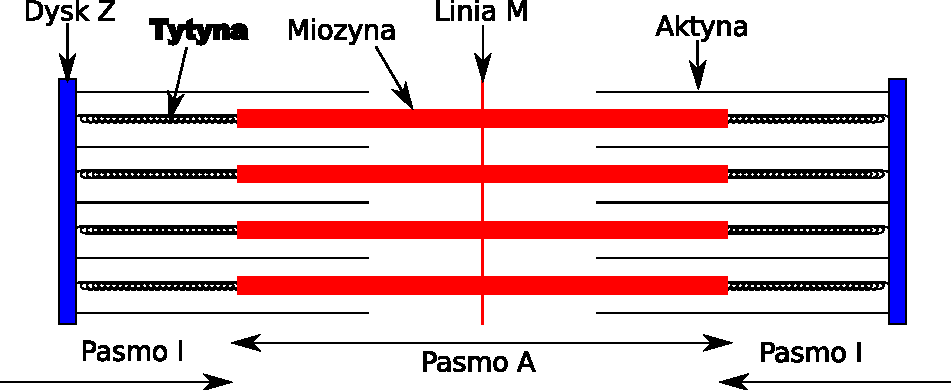
\includegraphics[width=300px]{./rys/sarko.pdf}
\caption{Schemat budowy sarkomeru.}
\end{centering}
\end{figure}

Tytyna składa się z około 300 powtórzeń domen fibrynokonektyny \mbox{typu~III~(Fn-3)}, która znajduje się tylko w paśmie A oraz domen immunoglobuliny (Ig), które występują wzdłuż całej jej długości. W skład wchodzi także obszar PEVK w pasmie I, który nie posiada jednej, stabilnej struktury. Długość regionu PEVK oraz ilość domen Ig w paśmie I waha się znacznie w zależności od miejsca występowania mięśnia poprzecznie prążkowanego w organizmie. Dla przykładu w mięśniach szkieletowych stwierdzono występowanie 90 domen Ig przy regionie PEVK składającym się z 2174 aminokwasów, kiedy w mięśniu sercowym wartości te wynoszą 37 domen Ig oraz 163 aminokwasów regionu PEVK\cite{Labeit_1995}.

\begin{figure}[h!]
\begin{centering}
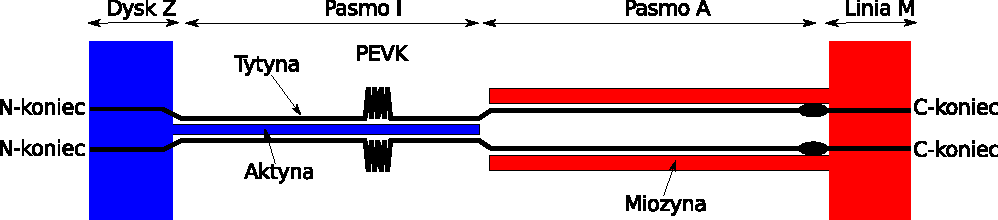
\includegraphics[width=400px]{./rys/tytyna.pdf}
\caption{Model tytyny w sakromerze.}
\end{centering}
\end{figure}

Podczas skurczu mięśnia tytyna odpowiada za utrzymanie elementów budulcowych sarkomeru. Podczas rozciągania natomiast gromadzi w sobie powstające naprężenia, przeciwdziała zerwaniu oraz powoduje powrót do stanu wyjściowego po ustaniu zewnętrznej siły powodującej rozciągnięcie. Stwierdzono, że obszar PEVK odpowiada za elastyczność tytyny przy niskich rozciągnięciach. Po rozwinięciu tego obszaru stabilnie pofałdowane domeny Ig stawiają opór dalszemu rozciąganiu powodując wzrost naprężenia. Tego typu mechanizm podwójnej sprężyny wyjaśnia niejednorodny wzrost naprężenia przy rozciąganiu pojedynczego sarkomeru.

W tej pracy szczególna uwaga poświęcona została kinazie tytyny, której struktura została dokładnie zbadana\cite{Tit_stru} oraz istnieje szereg publikacji z danymi eksperymentów AFM oraz symulacji dynamiki molekularnej\cite{mechanoenz, 1tki}. Białko to znajduje się blisko C-końca tytyny, w linii M. Polipeptyd ten składa się z 321 aminokwasów. Podczas powstawania naprężenia w mięśniu część tego naprężenia przekazywana jest na kinazę tytyny prowadząc do częściowego jej rozwinięcia, które powoduje odsłonięcie jej centrum aktywnego. Aktywna kinaza katalizuje fosforylację innego białka mięśniowego, telethoniny, które odgrywa rolę przy tworzeniu się mięśni, a także wpływa na ekspresję genów\cite{Kin_geny}. W ten sposób kinaza ta spełnia rolę molekularnego czujnika naprężenia.

\begin{figure}[h!]
\begin{centering}
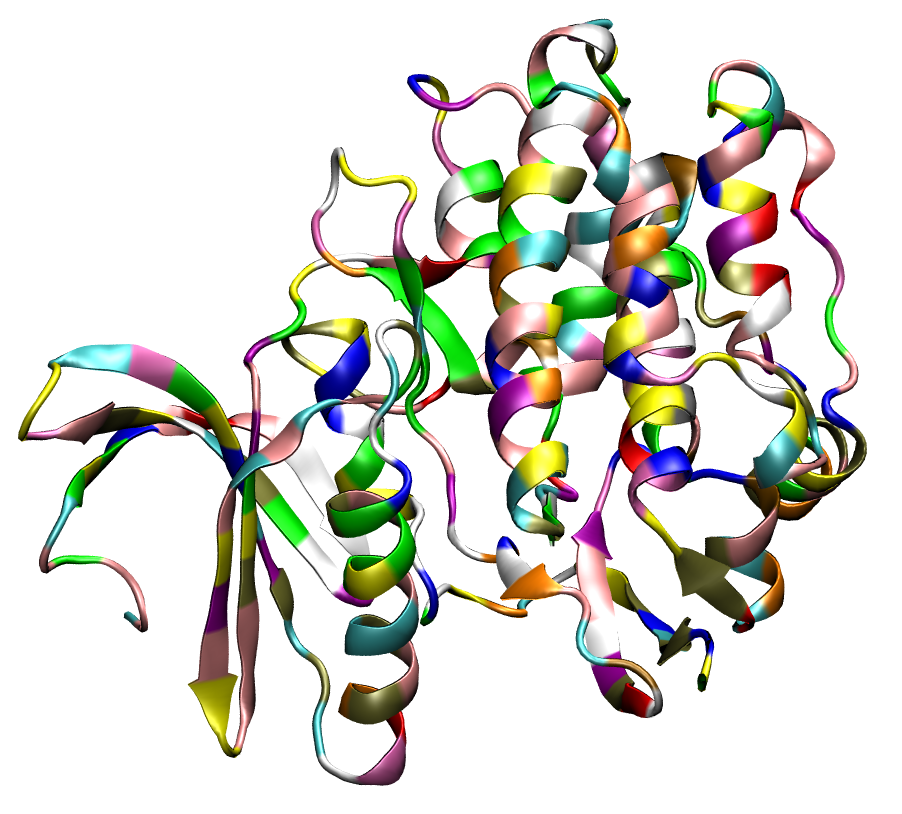
\includegraphics[width=300px]{./rys/plot_tki.png}
\caption{Wizualizacja struktury trzeciorzędowej domeny kinazy tytyny.}
\end{centering}
\end{figure}

\section{AFM}

Jednym z narzędzi, które pozwala na uzyskanie danych dla pojedynczych cząsteczek jest mikroskop sił atomowych (ang. Atomic Force Microscope --- AFM). W omawianych w tej pracy eksperymentach mamy do czynienia z cząsteczkami przytwierdzonymi do ostrza mikrodźwigni (ang. cantilever) z jednej strony, a do podstawy z drugiej. Następuje ruch podstawy w pionie i mierzone jest odchylenie sprężystego ramienia za pomocą wiązki laserowej. Na tej podstawie obliczana jest siła działająca na badaną cząsteczkę. W zależności od rodzaju eksperymentu możemy mieć do czynienia z rozciąganiem przy stałej sile, dzięki czemu można badać kinetykę reakcji w zależności od przyłożonego naprężenia\cite{Fernandez} albo przy stałej szybkości rozciągania, gdzie można badać miedzy innymi siły zerwania bądź też rozplatania\cite{Carrion-Vazquez30031999, Fisher1999379}. 

\begin{figure}[h]
\begin{centering}
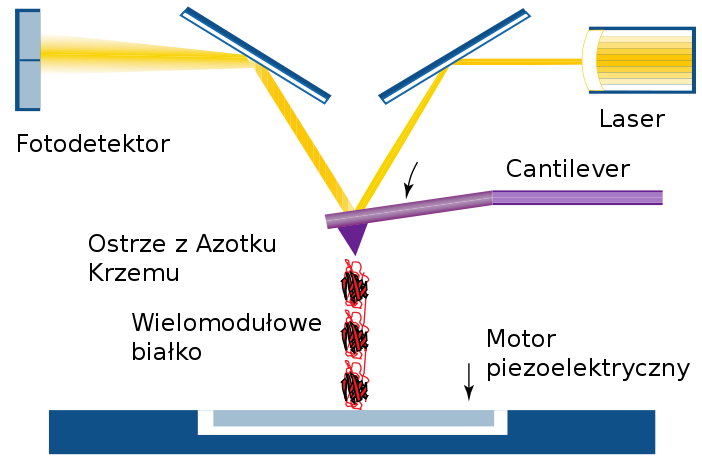
\includegraphics[width=300px]{./rys/afm1.png}
\caption{Schemat eksperymentu AFM.}
\end{centering}
\end{figure}

\section{Symulacje dynamiki molekularnej}

Symulacje dynamiki molekularnej (\textbf{MD} -- ang. Molecular Dynamics) stanowią jeden z działów chemii obliczeniowej (ang. Computational chemistry). W przeciwieństwie do symulacji Monte Carlo symulacje \textbf{MD} mogą być używane także do obliczeń układów nie będących w stanie równowagi oraz do wydarzeń dynamicznych, zachodzących w czasie. Z tego powodu symulacje \textbf{MD} są bardziej uniwersalne i znajdują zastosowanie w omawianym w tej pracy problemie\cite{Gromacs_manual}.

Podstawowym zadaniem, które stoi przed tymi obliczeniami jest rozwiązanie równań ruchu Newtona (\ref{eq:Newton}) dla układu składającego się z $N$ atomów oddziałujących na siebie zarówno za pomocą wiązań chemicznych jak i też za pomocą oddziaływań elektrostatycznych i van der Waalsa.

\begin{equation}m_{i}\frac{\partial ^{2}\vec{r_{i}}}{\partial t^{2}} = \vec{F_{i}}, \hspace*{0.5cm} \text{i}= 1 \ldots N \label{eq:Newton}\end{equation}

Gdzie $m_{i}$ oznacza masę, $\vec{r_{i}}$ wektor położenia, a $\vec{F_{i}}$ siłę działającą na \textit{i}-ty atom.

Dane na temat siły działającej na \textit{i}-ty atom znajduje się obliczając ujemny gradient z funkcji potencjału $V(\vec{r_{1}}, \vec{r_{2}}, \ldots, \vec{r_{N}})$

\begin{equation} \vec{F_{i}} = - \frac{\partial V(\vec{r_{i}})}{\partial \vec{r_{i}}} \end{equation}

Równania te rozwiązywane są numerycznie z małym krokiem czasowym. Co pewien czas w zależności od parametrów symulacji system jest kontrolowany pod względem temperatury oraz ciśnienia. Położenia oraz prędkości atomów są zapisywane w postaci trajektorii. Po początkowych dużych zmianach system po pewnym czasie osiąga stan równowagi. 

Symulacje te posiadają jednak pewne ograniczenia, z których należy zdawać sobie sprawę przy przeprowadzaniu i planowaniu obliczeń.
\begin{description}
\item[Symulacje odbywają się według mechaniki klasycznej] \hfill \\
Rozwiązując równania ruchu Newtona (\ref{eq:Newton}) pomijamy efekty kwantowe. Co za tym idzie symulacje \textbf{MD} nie nadają się do badania mechanizmów reakcji czy też stanów przejściowych. Istnieje jednak możliwość połączenia z programami do obliczeń kwantowomechanicznych, na przykład \textsc{Gaussian}, jednak obliczenia te są bardzo czasochłonne.
\item[Elektrony znajdują się w stanie podstawowym] \hfill \\
Wykorzystywane pola siłowe zawierają definicje oddziaływań atomów w stanie podstawowym. W obliczeniach nie uwzględnia się ruchu elektronów. Z tego powodu wszelkie procesy związane z transferem elektronów oraz te, gdzie stan wzbudzony odgrywa kluczową rolę w eksperymencie nie mogą być w pełni badane.
\item[Pola siłowe są tylko przybliżone] \hfill \\
Pola siłowe zawierają opis oddziaływań pomiędzy atomami w różnych cząsteczkach. Nie uwzględniają jednak możliwości polaryzacji wiązań. 
\item[Oddziaływania są w pewnej odległości ucinane] \hfill \\
Aby uprościć obliczenia oraz aby zapobiec nakładaniu się tych samych oddziaływań przez periodyczność stosuje się ograniczenie ich przy pewnej zdefiniowanej przez parametry symulacji odległości.
\item[Periodyczność pudła] \hfill \\
Aby zapobiec rozpraszaniu się atomów do próżni oraz aby uniknąć nienaturalnie małego układu badawczego wprowadzono periodyczność. Przez periodyczność w tym przypadku należy rozumieć fakt, że jeśli atom wybiega poza granice układu, to automatycznie pojawia się on po przeciwnej stronie. W ten sposób przenoszone są także oddziaływania pomiędzy atomami. Częściowo zbliża to badany układ do kryształu, co może powodować błędy w obliczeniach.
\end{description}
 

\subsection{Gromacs}\

Gromacs stanowi jeden z wielu dostępnych programów do symulacji dynamiki molekularnej, jednak ze względu na ilość materiałów szkoleniowych\cite{Gromacs_tut} i ilość publikacji, w których występuje, właśnie to narzędzie zostało użyte do obliczeń.

Gromacs stanowi pakiet programów do przygotowania symulacji, ich przeprowadzenia oraz analizy wyników. Dostępny jest bezpłatnie, na licencji GNU General Public License. Napisany został przez grupę Hermana Berendsensena (Department of Biophysical Chemistry of Groningen University). Obecnie rozwijany jest przez Erika Lindahla  (Stockholm Center for Biomembrane Research, SE), Davida van der Spoela (Biomedical Centre, Uppsala, SE) oraz Berka Hessa (Stockholm Center for Biomembrane Research, Stockholm, SE). 

Program został domyślnie napisany na systemy Uniksowe, jednak dostępny jest również pod system Windows. Spośród innych narzędzi wyróżnia się przede wszystkim wydajnością wynikającą ze zoptymalizowanego kodu, który wykorzystuje także multimedialne instrukcje procesorów jak MMX czy SSE (ang. Streaming SIMD Extensions) i SSE2. Przy wykorzystaniu bibliotek MPI (ang. Message Passing Interface) możliwe jest wykonywanie obliczeń na kilku jednostkach jednocześnie, co zdecydowanie skraca czas obliczeń. 

\subsection{NAMD}
W wielu publikacjach do symulacji używany jest program NAMD~\cite{NAMD}. Na stronie autorów \cite{namdtut} dostępne są tutoriale, które pozwalają na łatwiejsze wdrożenie się do pracy z tym programem. Jednak dla obliczeń prowadzonych przy zbliżonych warunkach NAMD okazuje się kilkukrotnie wolniejszy od programu \textsc{Gromacs}\cite{NAMD_sux}. Gromacs pozwala na zastosowanie dwukrotnie większego kroku czasowego przy tym samym błędzie obliczeń. Ponadto NAMD wykazuje gorszą skalowalność w porównaniu do Gromacsa i co za tym idzie obserwuje się większy spadek wydajności obliczeń na jednostkę obliczeniową przy wzroście liczby procesorów. Stąd też wybór programu Gromacs jako lepszego narzędzia do prowadzenia symulacji.

\section{Model teoretyczny Hummera-Szabo}

\begin{figure}[h]
\begin{centering}
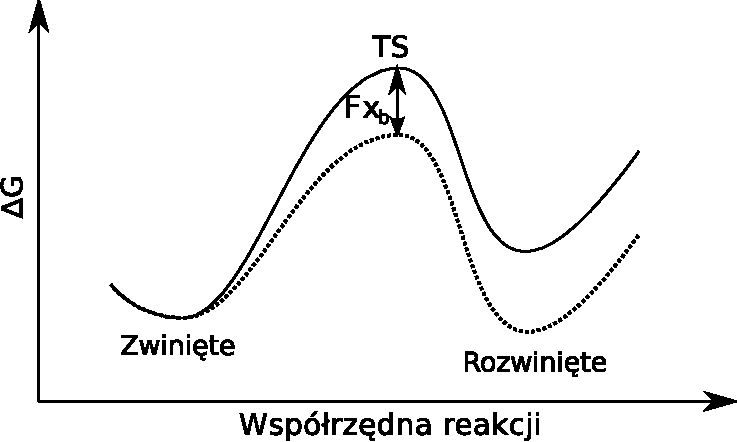
\includegraphics[width=100mm]{./rys/enswob.pdf}
\caption{Schemat ideowy zmiany powierzchni entalpii swobodnej pod wpływem rozciągania.}
\end{centering}
\end{figure}

Podczas rozciągania cząsteczki pod wpływem siły dochodzi do obniżenia bariery energetycznej stanu przejściowego, który cząsteczka musi przekroczyć by ulec rozwinięciu, które następuje w wyniku fluktuacji termicznych. Wprowadzenie siły do układu zwiększa prawdopodobieństwo przekroczenia bariery energetycznej. Do opisu fenomenologicznego tego zjawiska służy równanie Bell'a \ref{eq:bell}.

\begin{equation} k(t)=k_{0} \exp\left( \frac{ F(t)x_{b}}{k_{B}T}\right) \label{eq:bell}\end{equation}

Gdzie $k(t)$ oznacza stałą szybkości rozplatania przy sile $F(t)$, $k_{0}$ stanowi stałą szybkości rozplatania bez obecności siły, $x_{b}$ stanowi odległość bariery od minimum na powierzchni energii swobodnej, $k_{B}$ stanowi stałą Boltzmanna, a $T$ temperaturę bezwzględną.

Model fenomenologiczny zaprezentowany w pracy Hummera i Szabo \cite{Hummer_Szabo_2003} jest jednak niewystarczający do analizy wyników dla szerokiego zakresu szybkości rozciągania, ponieważ istniejące przybliżone rozwiązania analityczne mają zastosowanie tylko do wąskich, eksperymentalnych zakresów szybkości rozciągania i nie mogą być używane do analizy danych dla szybkości używanych w symulacjach.

W przypadku modelu mikroskopowego nie istnieją ścisłe rozwiązania analityczne, jednak przedstawione rozwiązanie numeryczne znajduje zastosowanie dla szerokiego zakresu prędkości. 

W modelu mikroskopowym zakładamy, że siła jest zdefiniowana potencjałem harmonicznym:

\begin{equation} V_{s}(x-vt)=\frac{1}{2} k_{B} T \kappa_{s}\left(x-vt\right)^2 \label{eq:harm}\end{equation}

Gdzie $V_{s}$ oznacza potencjał po współrzędnej reakcji $x$ (odległość ramienia od położenia 0), $v$ prędkość rozciągania, $t$ czas, a $\kappa_{s}$ oznacza stałą siłową wirtualnego cantilevera.

Kształt powierzchni entalpii swobodnej opisany jest zależnością:


\begin{equation} V_{0}(x)=\left\{
\begin{array}{l l} 
\frac{1}{2} k_{B} T \kappa_{m}x^2 & \quad \text{dla } x <  x_{b}\\
- \infty & \quad  \text{dla } x \geqslant x_{b}\\
\end{array} \right.
\label{eq:ent}\end{equation}

Gdzie $\kappa_{m}$ oznacza stałą sprężystości cząsteczki, a $x_{b}$ barierę, po której potencjał spada do $-\infty$.

System porusza się po następującej powierzchni potencjału: 

\begin{equation} V(x,t)=\left\{
\begin{array}{l l} 
\frac{1}{2} k_{B} T \kappa_{m}x^2 +\frac{1}{2} k_{B} T \kappa_{s}\left(x-vt\right)^2& \quad \text{dla } x <  x_{b}\\
- \infty & \quad  \text{dla } x \geqslant x_{b}\\
\end{array} \right.
\label{eq:potencjal_sum}\end{equation}

Zakładamy również, że system porusza się ruchem Browna po powierzchni potencjału wyznaczonej przez \ref{eq:potencjal_sum}. Wobec tego spełnione jest równanie dynamiki Browna:

\begin{equation} \dot{x}=-D \bigtriangledown V (x,t) +R(t)\label{eq:brown}\end{equation}

Gdzie $R(t)$ stanowi losową siłę z rozkładu Gaussa, gdzie jej wartość średnia wynosi 0, a wariancja $\overline{(t)R(t')}=2D\delta(t-t')$.

Po podstawieniu \ref{eq:potencjal_sum} do \ref{eq:brown} otrzymujemy równanie ruchu:

\begin{equation} \dot{x}=-D\kappa_{m} x - D\kappa_{s} (x-vt) +R(t)\label{eq:ruchu}\end{equation}

Przy założeniu, że $\overline{R(t)}=0$ można obliczyć $\overline{x}(t)$, oznaczające średnie położenie w chwili $t$, rozwiązując równianie \ref{eq:ruchu}, które przy pominięciu składnika $R(t)$ przy uśrednianiu przekształca się w równanie różniczkowe pierwszego rzędu. Równianie to rozwiązano przy użyciu programu Wolfram Alpha\cite{wolfram}. Jako rozwiązanie ogólne otrzymano:

\begin{equation} \overline{x}(t)= c_{1}e^{-(\kappa_{m}+\kappa_{s})Dt} + \frac{\kappa_{s}v((\kappa_{m}+\kappa_{s})Dt -1 )}{D(\kappa_{m}+\kappa_{s})^2} \label{eq:rozw_og}\end{equation}

Z warunku $\overline{x}(0)=0$ otrzymujemy współczynnik $c_1$ oraz rozwiązanie szczególne:

\begin{equation} \overline{x}(t)= \frac{\kappa_{s}v((\kappa_{m}+\kappa_{s})Dt + e^{-(\kappa_{m}+\kappa_{s})Dt}-1 )}{D(\kappa_{m}+\kappa_{s})^2} \label{eq:rozw_szczeg}\end{equation}

Aby znaleźć średnią siłę w danym czasie $\overline{F}(t)$ należy posłużyć się równaniem \ref{eq:harm} na zależność potencjału od czasu i położenia. W wyniku obliczenia ujemnej pochodnej po $x$ otrzymujemy siłę.

\begin{equation} \overline{F}(t) = - k_{B}t\kappa_{s} ( \overline{x}(t) -v t)  \label{eq:sila_czas}\end{equation}

Aby znaleźć średnią siłę zerwania należy przyjąć, że zerwanie następuje przy przejściu przez barierę $x_b$, które to następuje po czasie $\tau$. Czas ten można obliczyć z równania \ref{eq:rozw_szczeg} oraz warunku, że średnie położenie w momencie zerwania $\tau$ wynosi $x_b$, czyli $\overline{x}(\tau)=x_b$.

Aby znaleźć prawdopodobieństwo przeżycia systemu w czasie $t$, $S(t)$ czyli prawdopodobieństwo tego, że cząstka nie uległa rozpleceniu po czasie $t$ należy skorzystać z warunku:

\begin{equation} \dot{S}(t)=-k(t)S(t) \label{eq:surv_prob}\end{equation}

Dającego:

\begin{equation} S(t) = \exp\left( - \int_0^t k(t')dt' \right) \label{eq:surv_prob1}\end{equation}

Przy założeniu, że prędkość rozciągania jest na tyle niska, że energia aktywacji w trakcie rozplatania wciąż jest wysoka i nie ulega drastycznej zmianie, można użyć przybliżenia adiabatycznego $\Delta t=x(t)- \overline{x}(t)$, które prowadzi do wyrażenia:

\begin{equation} S(t) = \exp\left[ - \int_0^t k_{0}(x_b-\overline{x}(t'))dt' \right] \label{eq:surv_prob_corr}\end{equation}

Gdzie $k_0$ stanowi stałą szybkości uzyskaną z teorii Kramera:

\begin{equation} k_0(x_b)=\frac{1}{\sqrt{2\pi}}D\kappa_m^{3/2}x_b e^{-\kappa_mx_b^2/2} \label{eq:k_o}\end{equation}

Po podstawieniu \ref{eq:k_o} do \ref{eq:surv_prob_corr} otrzymuje się:

\begin{equation} S(t) = \exp\left[ - \frac{k_0 e^{-\kappa_s x_b^2 /2}}{v\kappa_s x_b (\kappa_m/(\kappa_m + \kappa_s))^{3/2}} (\exp(\kappa_s V x_b t -\frac{1}{2} (\kappa_s v t )^2 /(\kappa_m+ \kappa_s))-1) \right] \label{eq:s_t}\end{equation}

Wyrażenie to podstawione do:

\begin{equation} \overline{F}= - k_B T \kappa_s \left( x_b -v \int_o^\tau S(t)dt\right)\label{eq:wyn}\end{equation}

Pozwala na znalezienie zależności średniej siły rozplatania od prędkości rozciągania, $\overline{F}(v)$. Zależne jest ono od parametrów: $k_0$, $x_b$, oraz $\kappa_m$, które są dopasowywane do wartości sił rozplatania wziętych z symulacji dla różnych prędkości rozciągania.

\chapter{Cel pracy}
Cel pośredni pracy stanowiła symulacja rozplatania pojedynczego modułu kinazy tytyny przy różnych szybkościach rozciągania za pomocą programu Gromacs. Jako strukturę wyjściową wzięto strukturę krystalograficzną białka o symbolu 1TKI z bazy danych RCSB PDB \cite{pdbdb}. Wyniki symulacji zostały porównane z wynikami literaturowymi. 

Celem bezpośrednim było opracowanie uniwersalnej, niezależnej od badanej cząsteczki procedury numerycznej mającej za zadanie dopasowanie do danych z symulacji rozciągania krzywej teoretycznej z modelu mikroskopowego Hummera--Szabo\cite{Hummer_Szabo_2003}. Dopasowanie to pozwoliło na odzyskanie parametrów kinetycznych oraz porównanie wyników z danymi z eksperymentów AFM.

Podczas symulacji prowadzono także testy obliczeniowe klastra, dzięki czemu możliwa stała się analiza wydajności oraz ocena korzyści płynących z dalszej rozbudowy klastra.

Praca skaładała się z kilku etapów:
\begin{itemize}
\item Budowa klastra obliczeniowego
\item Symulacje
\begin{itemize}
\item Dobór parametrów symulacji
\item Równowagowanie
\item Właściwe obliczenia
\end{itemize}
\item Analiza wyników
\begin{itemize}
\item Odzyskanie sił rozplatania z wyników symulacji
\item Dopasowanie modelu do danych i odzyskanie parametrów kinetycznych
\end{itemize}
\item Wnioski
\end{itemize}

Praca ta ma także stanowić krótkie omówienie procedury przeprowadzania obliczeń programem Gromacs, kilku najważniejszych parametrów i problemów, które może napotkać początkujący użytkownik, tak aby zdobyta wiedza stanowiła w przyszłości punkt wyjścia dla będących zainteresowanymi rozpoczęciem pracy z tym programem.
\chapter{Metodologia pracy}
\section{Budowa i konfiguracja klastra}

Klaster obliczeniowy stanowi zespół komputerów połączonych w ten sposób, by prowadzić równolegle obliczenia, dzięki czemu czas potrzebny na ich wykonanie ulega skróceniu w porównaniu do pojedynczej jednostki obliczeniowej. Dzięki temu uzyskujemy wzrost wydajności bez potrzeby oczekiwania na coraz to nowszy sprzęt.

Budowany klaster składał się z dwóch dwuprocesorowych jednostek centralnych Dell Precision T5500, z czego każdy procesor posiadał 4 rdzenie. Razem daje to możliwość uruchomienia 16 niezależnych procesów. Specyfikacja sprzętu przedstawiona została w tabeli 4.1.

\begin{table}[ht!]
\centering
  \begin{tabular}{| r | p{10cm} |}
  \hline
  Podzespół & Opis \\
  \hline
 Procesor &  2 $\times$ Intel® Xeon® E5630; 4 rdzenie; 64 bit; taktowanie 2.53 GHz; 12 MB Cache \\
 Płyt główna & Intel® 5520 chipset; dwuprocesorowa\\
 Pamięć RAM & 12 GB; DDR3\\
 Dysk twardy & 500 GB; SATA\\
 karta sieciowa & Dwie karty sieciowe 1Gbps; jedna wbudowana na płycie głównej, druga w gnieździe PCI\\
 \hline  
  \end{tabular}
  \caption{Specyfikacja komputerów.}
\end{table}
Każdy z procesorów posiadał opcję HyperThreding, co pozwala na wirtualne podwojenie liczny rdzeni, jednak wcześniejsze obliczenia programem Gromacs pokazały, że włączenie opcji HT nie zwiększa wydajności obliczeń, a może ją wręcz zmniejszać w wyniku zwiększenia komunikacji pomiędzy wątkami przy dotychczasowej przepustowości.

Aby fizycznie zbudować klaster wystarczyło połączyć komputery do jednej sieci Ethernet za pomocą switcha (ośmioportowy D-link DGS-1008D 1000Mbps). Na tak połączonych komputerach należało następnie zainstalować system operacyjny. Ze względu na fakt, że pakiet Gromacs był domyślnie pisany pod systemy Uniksowe oraz rozpowszechnienie na pracowni wybór padł na system Ubuntu w serwerowej wersji 10.04 LTS (64 bit). Ponadto system ten jest darmowy oraz dobrze udokumentowany. Następnym etapem była instalacja bibliotek niezbędnych do działania Gromacsa na każdym z komputerów.

\subsection{Instalacja biblioteki OpenMPI}

Przy obliczeniach równoległych podstawowym problemem jest komunikacja pomiędzy poszczególnymi procesami (węzłami) klastra. W celu ułatwienia tworzenia programów działających równolegle stworzono na początku lat dziewięćdziesiątych protokół komunikacji \textbf{MPI} (ang. Message Passing Interface), który ze względu na rozpowszechnienie stał się standardem i występuje w postaci bibliotek dla różnych języków programowania i systemów operacyjnych. Protokół ten jest odpowiedzialny między innymi za zarządzanie pamięcią, synchronizację danych, komunikację pomiędzy procesami oraz rozdział procesów na poszczególne węzły. 

Również Gromacs korzysta ze standardu MPI. W związku z czym potrzebna była instalacja bibliotek obsługujących ten standard. Ze względu na rozpowszechnienie oraz na częste aktualizacje i szybkie poprawianie błędów wybrano bibliotekę OpenMPI w wersji 1.4.2, która dystrybuowana jest na licencji Open Source, dzięki czemu jest darmowa. Instalacja polega na ściągnięciu oraz rozpakowaniu archiwum z kodem źródłowym bibliotek, konfiguracji oraz kompilacji. Przy domyślnie zainstalowanym systemie instalacja sprowadza się do wykonania 3 podstawowych poleceń.
\begin{enumerate}
\item \texttt{./configure} -- uruchomienie skryptu konfiguracyjnego
\item \texttt{make} -- kompilacja
\item \texttt{make install} -- instalacja
\end{enumerate}
Przy konfiguracji należy pamiętać, by jako domyślną ścieżkę instalacji bibliotek podać katalog systemowy \texttt{/usr/lib}, po czym instalację wykonywać przy uprawnieniach superużytkownika (\texttt{sudo make install}). Dzięki temu uniknie się problemów przy dostępie do tych bibliotek przez inne programy i innych użytkowników.


\subsection{Instalacja biblioteki FFTW}
Kolejnym krokiem jest instalacja bibliotek do wykonywania transformaty Fourierowskiej. Ze względu na szybkość największą popularnością cieszy się biblioteka FFTW. Pomimo dostępności w repozytorium systemu Ubuntu zaleca się kompilację ze źródeł, ponieważ dzięki temu uwzględnia się wszystkie możliwe optymalizacje dostępne pod dany procesor, a nie tylko te najbardziej uniwersalne.

Do instalacji użyto biblioteki FFTW w wersji 3.2.2. Instalacja przebiega podobnie jak w przypadku OpenMPI. Domyślnie biblioteka ta kompiluje się w podwójnej precyzji, kiedy większość obliczeń Gromacsem odbywa się w pojedynczej precyzji, przez co podwójna precyzja biblioteki FFTW nie jest potrzebna. 

Kompilację i instalację prowadzi się przez wykonanie skryptu \texttt{./configure} z opcją \texttt{--enable-single}. Dzięki temu kompiluje się tę bibliotekę w pojedynczej precyzji. Ponadto można uwzględnić opcję obliczeń wielowątkowych dla systemów wielordzeniowych \texttt{--enable-threads} oraz instrukcje SSE dla rodziny procesorów i686 i nowszych \texttt{--enable-sse}.

Do poprawnej komunikacji pomiędzy programami wykorzystującymi bibliotekę OpenMPI na różnych komputerach wymagana jest możliwość zdalnego wywoływania poleceń na wszystkich komputerach wchodzących w skład klastra. Do tego celu służy protokół SSH (ang. \textit{Secure Shell}). Do obsługi wymagana jest instalacja serwera SSH na każdym z komputerów oraz możliwość bezhasłowego logowania się pomiędzy tymi węzłami. 

\subsection{Instalacja programu Gromacs}

Przy symulacjach użyto programu Gromacs w wersji 4.5.1. Jego instalacja jest zbliżona do instalacji bibliotek, jednak przy konfiguracji należy podać odpowiednie parametry do uzyskania wersji obsługującej obliczenia równoległe.

Dogodnie jest wykonać dwie instalacje. Jedną dla wersji bez obsługi protokołu MPI, a drugą z obsługą. Pierwszą instalację konfiguruje się standardowym skryptem \texttt{./configure} z podaniem ścieżki instalacji oraz wyborem zainstalowanej wersji bibliotek do transformaty fourierowskiej, w tym przypadku FFTW \texttt{--enable-fft=fftw3}. Całość kompiluje się poleceniem \texttt{make} oraz instaluje poleceniem \texttt{sudo make install} jeśli potrzeba, by program był dostępny dla wszystkich użytkowników oraz podana ścieżka instalacji nie znajduje się w katalogu użytkownika.

Aby dodać obsługę MPI przy konfiguracji należy podać opcję \texttt{--enable-mpi}. Aby rozróżnić instalację Gromacsa z MPI należy przy konfiguracji uwzględnić opcję, która do nazwy programu z obsługą MPI doda sufiks \_mpi \texttt{--program-suffix=\_mpi}. 

Poza głównym programem odpowiedzialnym za symulacje dynamiki pozostałe programy pakietu Gromacs nie korzystają z obsługi MPI, w związku z czym wystarczy skompilować i zainstalować tylko \texttt{mdrun} z obsługą MPI. Po konfiguracji służą do tego polecenia \texttt{make mdrun} oraz \texttt{sudo make install-mdrun}.

\section{Przygotowanie struktury do symulacji}
Jako przygotowanie cząsteczki do symulacji rozumie się wszelkie działania na plikach, podczas których nie wykonujemy obliczeń symulacji dynamiki molekularnej, które należy jednak przeprowadzić w celu uzyskania prawidłowej struktury wejściowej. Proces ten można rozbić na kilka najczęściej występujących etapów:
\begin{itemize}
\item Konwersja struktury na wewnętrzny format Gromacsa
\item Umieszczenie cząsteczki w pudełku
\item Dodatek wody do układu
\item Dodatek jonów do układu
\end{itemize}

Aby przeprowadzić symulację dynamiki danej cząsteczki należy dysponować jej strukturą, którą uzyskuje się w wyniku badań krystalograficzncyh lub NMR. W internecie istnieje otwarta i darmowa baza danych z rozwiązanymi strukturami białek, RCSB Protein Data Bank \cite{pdbdb}, z której można pobrać plik w formacie PDB.

Jeśli badane białko zawiera aminokwasy kwasowe bądź zasadowe, to należy pamiętać, że różne stany sprotonowania prowadzą do różnej struktury, co może mieć wpływ na otrzymane wyniki. W celu optymalizacji struktury należy posłużyć się programem WHATIF, który jest dostępny w postaci usługi sieciowej z poziomu przeglądarki internetowej \cite{WHATIF}. W pliku PDB zawierającym definicję białka 1TKI należało ręcznie usunąć linie zawierające wpisy położeń wody krystalizacyjnej oraz jednego z dwóch łańcuchów.

Posiadając już odpowiedni plik PDB należy przekonwertować go na wewnętrzny format używany przez Gromacsa. Do tego celu służy jeden z programów pakietu Gromacs, mianowicie \textsf{pdb2gmx}. W wyniku jego działania otrzymujemy plik \texttt{.gro} zawierający informacje o wielkości pudła, liczbie atomów w układzie, ich położeniach i prędkościach oraz plik z topologią \texttt{.top}, w którym znajdują się definicje typów atomów, ich masy, ładunki, typy wiązań oraz definicje oddziaływań i odwołania do pól siłowych.

Pole siłowe stanowi bazę zawierającą definicje dla ładunków cząstkowych atomów, długości wiązań, ich stałych siłowych, oraz innych oddziaływań dla różnego typu cząsteczek (ang. \textit{residues}) takich jak aminokwasy, nukleotydy, cukry czy też parametry dla jonów. W zależności od dokładności definicji atomów pola siłowe dzielimy na pola typu \textit{all atom}, które zawierają definicje dla ładunków oraz oddziaływań dla wszystkich atomów występujących w cząsteczce oraz na pola typu \textit{united atom}, które pomijają definicje dla atomów wodorów niepolarnych. Jeśli zamierza się symulować dynamikę cząsteczek nieujętych w definicji pola siłowego należy uzyskać na podstawie obliczeń kwantowomechanicznych ładunki cząstkowe oraz parametry dla oddziaływań w cząsteczce i dodać tę definicję. Komplikuje to używanie programów \textbf{MD} do niestandardowych układów.

Program używany do konwersji, \texttt{pdb2gmx} pozwala na wybór pola siłowego, modelu wody oraz stanu sprotonowania poszczególnych aminokwasów. Do symulacji użyto pola siłowego GROMOS, które jest polem typu \textit{united atom} oraz modelu wody SPC. Stany sprotonowania histydyn zostały wybrane w oparciu o strukturę w pliku PDB otrzymanego w wyniku użycia programu WHATIF. Program ten dodaje również atomy wodoru nie wykryte podczas ustalania struktury. Wybrane pole siłowe nie zawiera definicji wszystkich atomów wodorów występujących w strukturze w pliku PDB, co prowadzi do błędów podczas konwersji na format plików Gromacsa. Aby temu zapobiec stosuje się program \texttt{pdb2gmx} z opcją \texttt{-ignh}, która powoduje pobranie informacji o położeniach atomów wodoru nie z pliku PDB, ale z definicji pola siłowego. Dodatkowa opcja \texttt{-his} pozwala na interaktywny wybór stanu sprotonowania histydyny, dzięki czemu informacja o wodorach biorących udział w tworzeniu wiązań wodorowych nie jest tracona.

Aby zdefiniować rozmiary pudełka wykorzystuje się kolejny z programów Gromacsa, \texttt{editconf}. Początkowe wymiary pudełka obieramy na podstawie publikacji\cite{1tki} na 8.8 x 7.8 x 7.6 nm. Białko umieszcza się w pudełku poleceniem \texttt{editconf} z parametrami pliku wejściowego, wyjściowego oraz opcją \texttt{-box 8.8 7.8 7.6} określającą wymiary w nm oraz \texttt{-c} umieszczającą środek geometryczny białka w środku pudełka.

Kolejnym etapem jest dodatek cząsteczek wody do układu. Gromacs zawiera zdefiniowane kilka różniących się od siebie modeli wody:
\begin{itemize}
\item \textbf{SPC} --- prosty, trójpunktowy model wody
\item \textbf{SPC/E} --- rozszerzony trójpunktowy model wody
\item \textbf{TIP3P} --- trójpunktowy model wody stosowany w polach siłowych CHARMM i AMBER
\item \textbf{TIP4P} --- czteropunktowy model wody, gdzie 3 punkty stanowią atomy tlenu i wodoru, natomiast czwarty punkt stanowi zdelokalizowany ładunek. Stosowany najczęściej dla pola siłowego OPLS/AA
\item \textbf{TIP5P} --- model pięciopunktowy, gdzie dwa dodatkowe punkty odpowiadają definicjom wolnych par elektronowych tlenu
\end{itemize}
Chcąc powtórzyć wyniki pracy \cite{1tki} wybrano model SPC.

Do addycji wody do układu służy program \texttt{genbox}. W linii poleceń oprócz pliku wejściowego, wyjściowego oraz pliku z topologią należy podać plik ze strukturą wody, która zostanie powielona. W tym przypadku definicje wody znajdują się w pliku \texttt{spc216.gro} znajdującym się w katalogu głównym Gromacsa. W wyniku działania programu otrzymuje się układ składający się z 49606 atomów. 

Następnie należało dodać do układu jony w celu zrównoważenia ładunku +2e białka oraz aby zbliżyć układ do warunków eksperymentalnych. Wykorzystuje się do tego program \texttt{genion}, będący częścią składową Gromacsa. Przed jego użyciem należy posiadać plik wsadowy do symulacji \texttt{.tpr}, który generuje się komendą \texttt{grompp}. Jako plik z parametrami posłużył plik do minimalizacji energii \texttt{em.mdp}. Posiadając już plik wsadowy należy w poleceniu \texttt{genion} podać go jako plik wejściowy, podać plik wyjściowy, plik z topologią oraz opcją \texttt{-nn} liczbę jonów ujemnych oraz \texttt{-np} liczbę jonów dodatnich. Jako domyślne program ten bierze kationy sodu oraz aniony chlorkowe, których liczba wynosi odpowiednio 29 i 27.

Istnieje również możliwość ustalenia stężenia jonów za pomocą opcji \texttt{-conc} w mol/litr oraz opcji \texttt{-neutral}, która odpowiada za otrzymanie układu elektrycznie obojętnego.

Mając tak zdefiniowany układ można przejść do właściwego etapu, jakim jest symulacja.

\section{Równowagowanie}

\begin{figure}[h!]
\begin{centering}
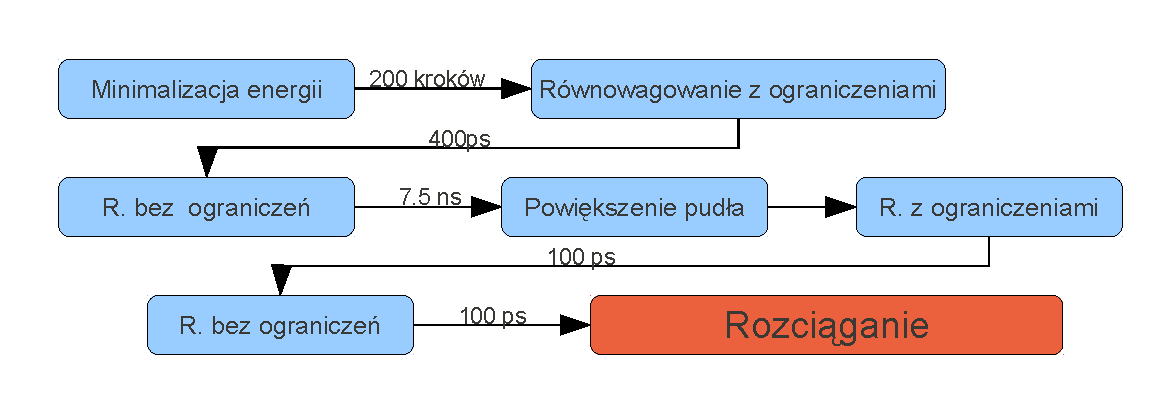
\includegraphics[width=150mm]{./rys/schemat.pdf}
\caption{Schemat przebiegu równowagowania i symulacji.}
\end{centering}
\end{figure}

Przed właściwą symulacją należy przeprowadzić równowagowanie całego układu tak, aby wyeliminować w jak największym stopniu różnice między układem symulowanym, a rzeczywistym. Różnice te wynikają przede wszystkim z faktu, że dysponujemy strukturą krystaliczną, która nie odpowiada w pełni strukturze białka w roztworze, do której dąży się poprzez równowagowanie.


\subsection{Minimalizacja energii}

Pierwszym etapem jest minimalizacja energii całego układu. W wyniku dodawania wody, jonów, a także nieprawidłowości w samej strykturze pliku PDB mogą powstać miejsca, w których atomy znajdują się zbyt blisko siebie lub wręcz nakładają się wiązaniami. Podczas swobodnej symulacji prowadziłoby to do nadania tym atomom znacznie zawyżonych wartości energii kinetycznych, przez co badany układ by się rozpadł. Zjawisko to nazywa się eksplozją układu.

W celu ograniczenia tego efektu prowadzi się minimalizację energii potencjalnej układu. W wyniku tej operacji otrzymuje się układ o jak najmniejszych oddziaływaniach pomiędzy atomami. 

W tym celu utworzono plik z parametrami symulacji \texttt{em.mdp}. Najważniejsze na tym etapie parametry, które służą do kontroli symulacji to wybór integratora czyli algorytmu obliczeniowego oraz nadanie wartości specyficznym dla niego parametrom. W przypadku minimalizacji energii najczęściej wykorzystywanym i najszybszym, ale mało dokładnym algorytmem jest metoda najszybszego spadku. Do jej wyboru służy opcja \texttt{integrator = steep}. Dla tej metody charakterystyczne są parametry:
\begin{itemize}
\item \texttt{emtol} --- Określa maksymalną siłę, poniżej której optymalizacja jest uznana za zakończoną.
\item \texttt{nsteps} --- Maksymalna liczba kroków optymalizacji.
\item \texttt{emstep} --- Krok.
\end{itemize}

Posiadając już plik \texttt{.mdp} wraz ze strukturą oraz topologią należy stworzyć binarny plik wejściowy z rozszerzeniem \texttt{.tpr} dla właściwych obliczeń. Służy do tego program \texttt{grompp}. 

\texttt{grompp -f em -o em -c ions.gro -p topol}

Posiadając już plik \texttt{em.tpr} można uruchomić właściwą symulację. Służy do tego polecenie \texttt{mdrun}. Jednak ze względu na używaną wielowątkowość należy poprzedzić je poleceniem środowiska OpenMPI \texttt{mpirun}.

Do poprawnego działania wymaga ono podania liczby uruchamianych procesów \texttt{-np 16}, od 16 uruchamianych procesów oraz adresów sieciowych komputerów, na których prowadzone będą obliczenia. Można je podać bezpośrednio w linii komend, jednak wygodniej jest umieścić je w pliku, który wskazuje się opcją \texttt{-machinefile}. Na strukturę tego pliku składają się adresy sieciowe lub nazwy hostów komputerów. Opcjonalnie można po spacji podać maksymalną liczbę możliwych do uruchomienia wątków na danym komputerze, w tym przypadku było to 8 \texttt{max-slots=8} oraz liczbę wątków, które mają zostać wykorzystane, \texttt{slots=8}. Po zapisaniu tych linii do pliku \texttt{hosts}, komenda wygląda następująco:

\texttt{mpirun -np 16 -hostfile ./hosts mdrun\_mpi -v -deffnm em}

W wyniku obliczeń uzyskuje się kilka plików z następującymi rozszerzeniami:
\begin{itemize}
\item \texttt{.log} --- Zawiera podsumowanie obliczeń
\item \texttt{.edr} --- Plik z wartościami ciśnienia, temperatury, objętości, wyszczególnionych energii i innymi parametrami w zależności czasowej.
\item \texttt{.trr} --- plik z trajektorią. Przez trajektorię rozumie się położenia atomów oraz ich prędkości w zależności od czasu.
\item \texttt{.gro} --- Struktura po optymalizacji.
\end{itemize}

Korzystając z programu \texttt{g\_energy} można pokazać jak zmieniała się energia potencjalna całego układu wraz z postępem optymalizacji. Na wykresie widać szybki spadek energii potencjalnej na początku minimalizacji oraz niewielkie jej zmiany pod koniec.

\begin{figure}[h]
\begin{centering}
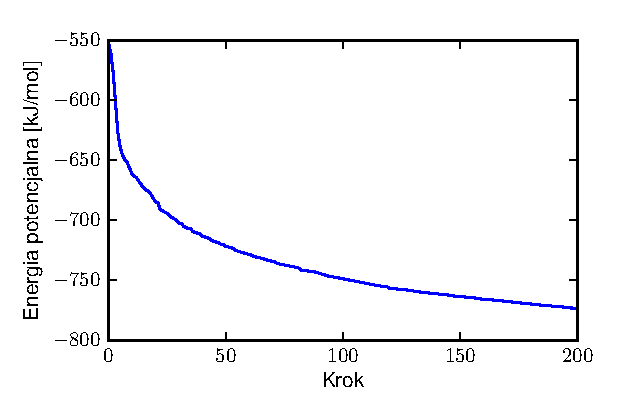
\includegraphics[width=100mm]{./rys/em_pot.pdf}
\caption{Energia potencjalna układu podczas minimalizacji.}
\end{centering}
\end{figure}

\subsection{Równowagowanie rozpuszczalnika}

Kolejnym krokiem w równowagowaniu jest już właściwa symulacja z ograniczeniami nałożonymi na atomy białka tak, by nie zmieniły one swojego położenia. Pozawala to na swobodne rozmieszczenie rozpuszczalnika wraz z jonami wokół białka. Podczas tworzenia topologii przy konwersji z pliku PDB automatycznie tworzony jest plik z ograniczeniami (\texttt{.itp}) dla każdego atomu białka. Jego definicja jest automatycznie dodawania do pliku topologii, jednak domyślnie jest on nieaktywny. Można go aktywować w pliku \texttt{.mdp} dodając linię \texttt{define = -DPOSRES}. Nakłada on na każdy atom białka potencjał harmoniczny ze stałą siłową domyślnie 1000~kJ~mol$^{-1}$~nm$^{-2}$ w każdym z wymiarów przestrzennych. Dzięki temu próba przesunięcia atomu w którymkolwiek kierunku prowadzi do niekorzystnego, wyższego stanu energetycznego układu. Metoda ta ma tę zaletę, że nie prowadzi do całkowitego unieruchomienia wybranych atomów. 

W przypadku właściwej symulacji najczęściej stosowanym integratorem jest \texttt{md}. Tak też jest w tym przypadku. Do najważniejszych parametrów tej opcji należy krok czasowy \texttt{dt} [ps], który po zastosowaniu dalszych algorytmów optymalizacyjnych może być zmniejszony do 2~fs. Mając już ustalony krok czasowy oraz znając czas trwania symulacji można podać jako parametr \texttt{nsteps} liczbę kroków symulacji. W przypadku symulacji trwającej 400~ps liczbę kroków ustalono na 200000. 

Grupa parametrów z prefiksem \texttt{nst} opisuje częstość zapisu wartości takich jak położenia atomów, ich prędkości, energie czy też zwykłe informacje kontrolne na temat symulacji do plików. Zawiera informację co ile kroków parametry te są zapisywane. Ma to wpływ na rozdzielczość późniejszych danych do analizy oraz ilość przestrzeni dyskowej zajmowanej przez zapisaną trajektorię. 

Rozpoczynając symulację należy nadać prędkości początkowe atomom. Służy do tego parametr \texttt{gen\_vel}, który przyjmuje wartości \texttt{yes} albo \texttt{no}. Prędkości dobierane są losowo z rozkładu Maxwella do temperatury podanej w parametrze \texttt{gen\_temp} [K]. Do ustalenia ziarna służy parametr \texttt{gen\_seed}, który ustawiony na \texttt{-1} przybiera wartość automatyczną na podstawie numeru procesu w systemie. Chcąc kontynuować symulację z nowymi parametrami należy pamiętać, by w nowym pliku \texttt{.mdp} ustawić \texttt{gen\_vel} na \texttt{no}. Zapobiegnie to nadaniu nowych prędkości już zrównowagowanemu układowi.

\subsection{Termostat}

Kolejną kwestią jest kontrola temperatury. W wyniku zmniejszonej precyzji obliczeń oraz błędów numerycznych temperatura układu może ulegać znacznym fluktuacjom. Aby tego uniknąć stosuje się algorytmy kontroli stałości temperatury zwane termostatami. W tym przypadku układ równowagowany był do stałej temperatury 300~K. 

Gromacs oferuje do wyboru trzy algorytmy kontroli temperatury (\texttt{berendsen}, \texttt{V-rescale} oraz \texttt{nose-hoover}) określane parametrem \texttt{tcoupl}, gdzie \texttt{no} oznacza brak termostatu. 

Termostat Berendsena stanowi algorytm prostego skalowania prędkości wszystkich cząsteczek w danej grupie. Jako parametr opisujący szybkość doprowadzania układu do zadanej temperatury służy \texttt{tau\_t}, natomiast temperaturę układu, do której się dąży opisuje \texttt{ref\_t}. Aby uniknąć sytuacji, kiedy to większość energii kinetycznej przekazywana jest do rozpuszczalnika, prowadząc do problemu gorącego rozpuszczalnika i zimnej substancji rozpuszczonej zaleca się oddzielne sprzęganie rozpuszczalnika i substancji rozpuszczonej. Grupy te definiuje się parametrem \texttt{tc\_grps} rozdzielając je spacją i podając temperaturę dla każdej z nich.

Termostat Berendsena jest najszybszy, jednak może prowadzić do powstawania błędów, gdyż nie uwzględnia rozkładu statystycznego skalowanych prędkości. Dlatego też w nowszej wersji programu Gromacs zaleca się stosowanie termostatu V-rescale, który jest zmodyfikowanym termostatem Berendsena, w ten sposób,  że uwzględnia poprawny rozkład energii kinetycznej w układzie.

Algorytm Nosé-Hoover jest najwolniejszym, ale też najdokładniejszym z omawianych algorytmów. Pozwala na fluktuację temperatury wokół danej wartości. Jeśli poprzednie dwa termostaty pozawalają na szybkie doprowadzenie układu do pożądanej temperatury, tak ten termostat pozawala na najbardziej wierne jej zachowanie w trakcie symulacji. Jednak w publikacji, na którą się powołano próbując odtworzyć wyniki \cite{1tki} używa się termostatu Berendsena przy temperaturze 300 K oraz stałej sprzęgania $\tau_{T}$=0.1~ps, przez co w symulacjach użyto termostatu V-rescale.

\subsection{Barostat}

Mając ściśle zdefiniowane, stałe początkowe wymiary pudełka traci się kontrolę nad ciśnieniem oraz nad gęstością układu. Aby jak najbardziej zbliżyć symulację do rzeczywistego eksperymentu wprowadzono kontrolę ciśnienia poprzez stosowanie barostatów parametrem \texttt{pcoupl}. Najczęściej stosowanymi dwoma algorytmami są \texttt{berendsen} oraz \texttt{parrinello-rahman}.

Tak jak w przypadku termostatu algorytm Berendsena stanowy szybki i prosty algorytm skalowania, w tym przypadku wymiarów pudełka tak, by doprowadzić ciśnienie układu do pożądanej wartości. Może to prowadzić do błędów, ponieważ nie odwzorowuje prawidłowo układu stałej liczby atomów, ciśnienia i temperatury (NPT). W tym celu lepszym rozwiązaniem jest stosowanie algorytmu Parrinello-Rahmana, jednak należy pamiętać, że działanie tego algorytmu opiera się na oscylacji wokół stałego ciśnienia, co przy początku symulacji z dużej różnicy ciśnień może doprowadzić do nadania atomom niebezpiecznie wysokich prędkości. W omawianej symulacji używa się algorytmu Berendsena.

Do kontroli stałego ciśnienia służą następujące parametry:
\begin{itemize}
\item \texttt{pcoupltype} --- Definiuje rodzaj skalowania pudełka. Najczęściej używanymi są \texttt{isotropic}, gdzie pudełko jest skalowane we wszystkich wymiarach tak samo, \texttt{semiisotropic}, gdzie skalowanie w wymiarze \texttt{x} oraz \texttt{y} jest takie samo, natomiast wymiar \texttt{z} skalowany jest niezależnie (zastosowanie przy symulacji błon lipidowych) oraz \texttt{anisotropic}, gdzie każdy z wymiarów jest skalowany niezależnie, a ponadto skalowane są dodatkowo 3 kierunki diagonalne.
\item \texttt{tau\_p} --- Określa stałą czasową relaksacji $\tau_{p}$ w symulacji określoną jako 1.0~ps.
\item \texttt{ref\_p} --- Określa ciśnienie do którego sprzęgany jest układ. Należy zdefiniować każdy wymiar. Aby w skalowaniu anizotropowym uniknąć skalowania ciśnienia w kierunkach diagonalnych ustala się ciśnienie na 0. Dzięki temu symulowane pudełko nie przekształca się w pudełko trygonalne. W pozostałych wymiarach ciśnienie ustala się na 1.0~bar.
\item \texttt{compressibility} --- Ściśliwość, ustalana w każdym z wymiarów, domyślnie dla wody wynosi 4.5$\times10^{-5}$~bar$^{-1}$. Tak jak w przypadku ciśnienia należy również ustalić 0 dla diagonalnych.
\end{itemize}

Wszystkie parametry dla tego etapu symulacji umieszczono w pliku \texttt{npt\_res.mpd}. Posiadając już ten plik można zastosować polecenia z wcześniejszego etapu. Całość tego symulacji zajęła 48~min~40~s na 16 rdzeniach. 

\subsection{Równowagowanie układu}

Posiadając już strukturę z poprzedniej symulacji można przejść po usunięciu ograniczeń nałożonych na atomy białka do etapu równowagowania całego układu. Dzięki temu struktura krystaliczna białka zbliży się do tej, która występuje w roztworze. 

Po usunięciu ograniczeń położenia atomów białka mogą one w wyniku drgań termicznych ulegać zmianie, w wyniku czego całe białko ulega rotacji i translacji. W wyniku określenia periodyczności układu nie stanowi to problemu podczas równowagowania, jednak przygotowując białko do rozciągania należy to uwzględnić w dalszej symulacji.

Aby mimo wszystko zachować położenie białka w centrum i pozwolić na ustalenie się struktury trzeciorzędowej zbliżonej do tej występującej w roztworze należy usunąć ruch środka ciężkości białka. W tym celu należy zdefiniować w pliku \texttt{mdp} parametr \texttt{comm\_mode} jako \texttt{Linear}, który usuwa ruch translacyjny środka masy, \texttt{Angular}, który usuwa ruch translacyjny jak i rotację cząsteczki lub grupy cząsteczek wokół środka masy lub \texttt{No}.

Tryb \texttt{Linear} może być użyty w obliczeniach wielowątkowych, podczas których zachodzi podział pudełka na obszary, które liczą się oddzielnie (\textit{domain decomposition}), natomiast tryb \texttt{Angular} może być użyty tylko w trybie \textit{particle decomposition}, co oznacza podział nie na obszary, ale na cząsteczki liczone na oddzielnych wątkach. Dlatego też aby przyspieszyć obliczenia nie ustalano parametru \texttt{comm\_mode} w pliku \texttt{.mdp}, dzięki czemu Gromacs automatycznie ustawił go na usuwanie ruchu translacyjnego środka masy umożliwiając tym samym tryb pracy \textit{domain decomposition}.

Równowagowanie prowadzone było przez 7.5~ns, gdzie czas obliczeń na 16 rdzeniach wyniósł 13h 38min 15s.

Do kontroli procesu równowagowania służy obserwacja temperatury i ciśnienia układu, a także RMSD (root-mean-square deviation) czyli pierwiastka ze średniej kwadratów odchyleń położeń atomów od położenia początkowego dla łańcucha głównego białka. Do uzyskania tych danych z obliczonej trajektorii służą polecenia \texttt{g\_rms} oraz \texttt{g\_energy}. Jako parametry wejściowe polecenia te biorą plik \texttt{.tpr} oraz odpowiednio trajektorię \texttt{.trr} lub \texttt{.xtc} oraz plik z danymi o układzie \texttt{.edr}. Na wyjściu otrzymuje się pliki w formacie \texttt{.xvg}, które można otwierać bezpośrednio programem \texttt{xmgrace} lub też jak w tym przypadku poddawać je analizie w innym środowisku, na przykład Python.


\begin{figure}[h]
\begin{centering}
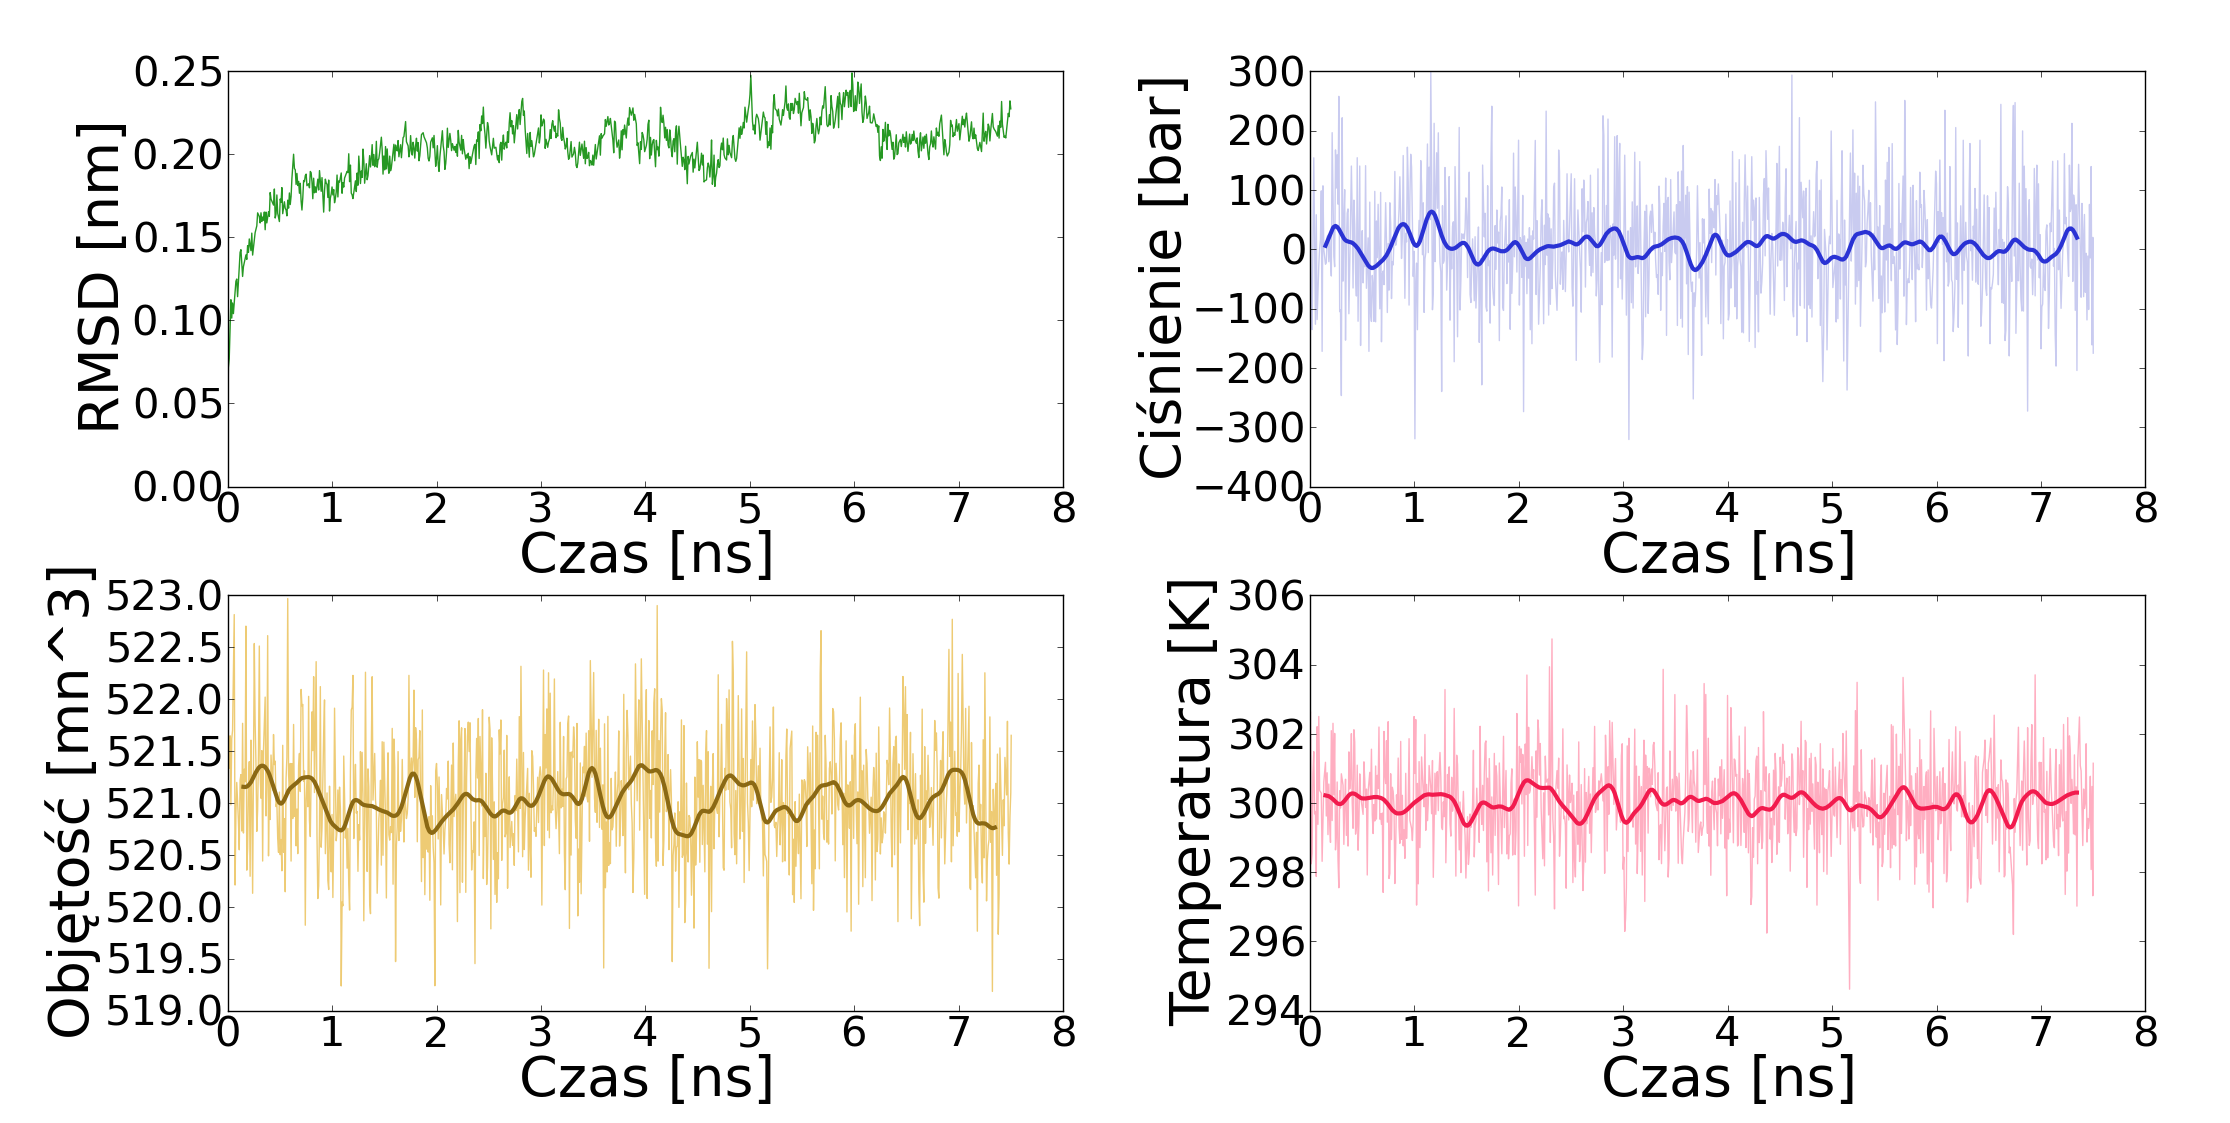
\includegraphics[width=150mm]{./rys/rmsd.png}
\caption{Zmiana RMSD, ciśnienia, objętości i temperatury w czasie podczas równowagowania.}
\end{centering}
\end{figure}


Analiza wykresów p, T i V wskazuje na ustalenie się ich wartości i fluktuację wokół zadanych parametrów, co jest zachowaniem pożądanym. Wykres RMSD także szybko rośnie do pewnego momentu, po czym nie przekracza wartości 0.25 nm, dzięki czemu można domniemywać, że białko osiągnęło strukturę równowagową. Dysponując ograniczonym czasem na wykonanie obliczeń trzeba polegać na założeniu wiarygodności tych danych, którymi się dysponuje, gdyż nigdy nie wiadomo jakim zmianom strukturalnym podlegałoby białko w dalszym czasie.

W wyniku równowagowania bez usuwania rotacji wokół środka ciężkości białka uległo ono obróceniu. Przy symulacji rozciągania jest to niekorzystne, ponieważ należałoby zastosować pudełko sześcienne, które przez zwiększoną objętość powodowałoby zwiększenie czasu obliczeń. Aby tego uniknąć stosuje się pudełko w formie prostopadłościanu o wymiarze zwiększonym tylko w kierunku rozciągania tak, aby pomieścić rozwijane białko. 

W tym celu w dalszym etapie należy białko obrócić tak, by zorientować N i C-koniec białka wzdłuż jednej z osi układu współrzędnych i stworzyć nowe pudełko. 

Służy do tego skrypt napisany w środowisku programistycznym Python (rot.py), który wczytuje plik \texttt{.gro} oraz oblicza kąty pomiędzy wektorem utworzonym pomiędzy dwoma zadanymi atomami, a osiami układu współrzędnych. W przypadku 1TKI atomami tymi były atomy węgla alfa Ile 138 oraz Lys 18. Mając już wartości kątów, korzysta się z polecenia \texttt{editconf} z parametrem \texttt{-rotate}, po którym podaje się kąty w stopniach, o które należy obrócić cząsteczkę wokół osi X Y Z tak, by wybrane wcześniej atomy znalazły się wzdłuż osi Z, po której białko ulega rozciągnięciu. 

Po obrocie pudełka usunięto rozpuszczalnik oraz jony z układu zarówno w pliku \texttt{gro} jak i pliku z topologią. Następnie stworzono nowe pudełko o wymiarach 7.8 x 8.4 x 18.6 nm, dodano rozpuszczalnika oraz jonów według procedury opisanej poprzednio, co w efekcie dało 119587 atomów w układzie. Ponownie równowagowano układ najpierw z ograniczeniami nałożonymi na atomy białka, a następnie bez ograniczeń przez 100~ps. Czas obliczeń na 16 rdzeniach wyniósł odpowiednio 27min 10s oraz 28min 6s. Dzięki tej procedurze równowagowanie białka mogło być przeprowadzone w mniejszym pudełku, a co za tym idzie obliczenia trwały krócej niż miałoby to miejsce przy równowagowaniu przez 7.5~ns przy wymiarach pudełka niezbędnych do symulacji rozciągania. 


\begin{figure}[h]
\begin{centering}
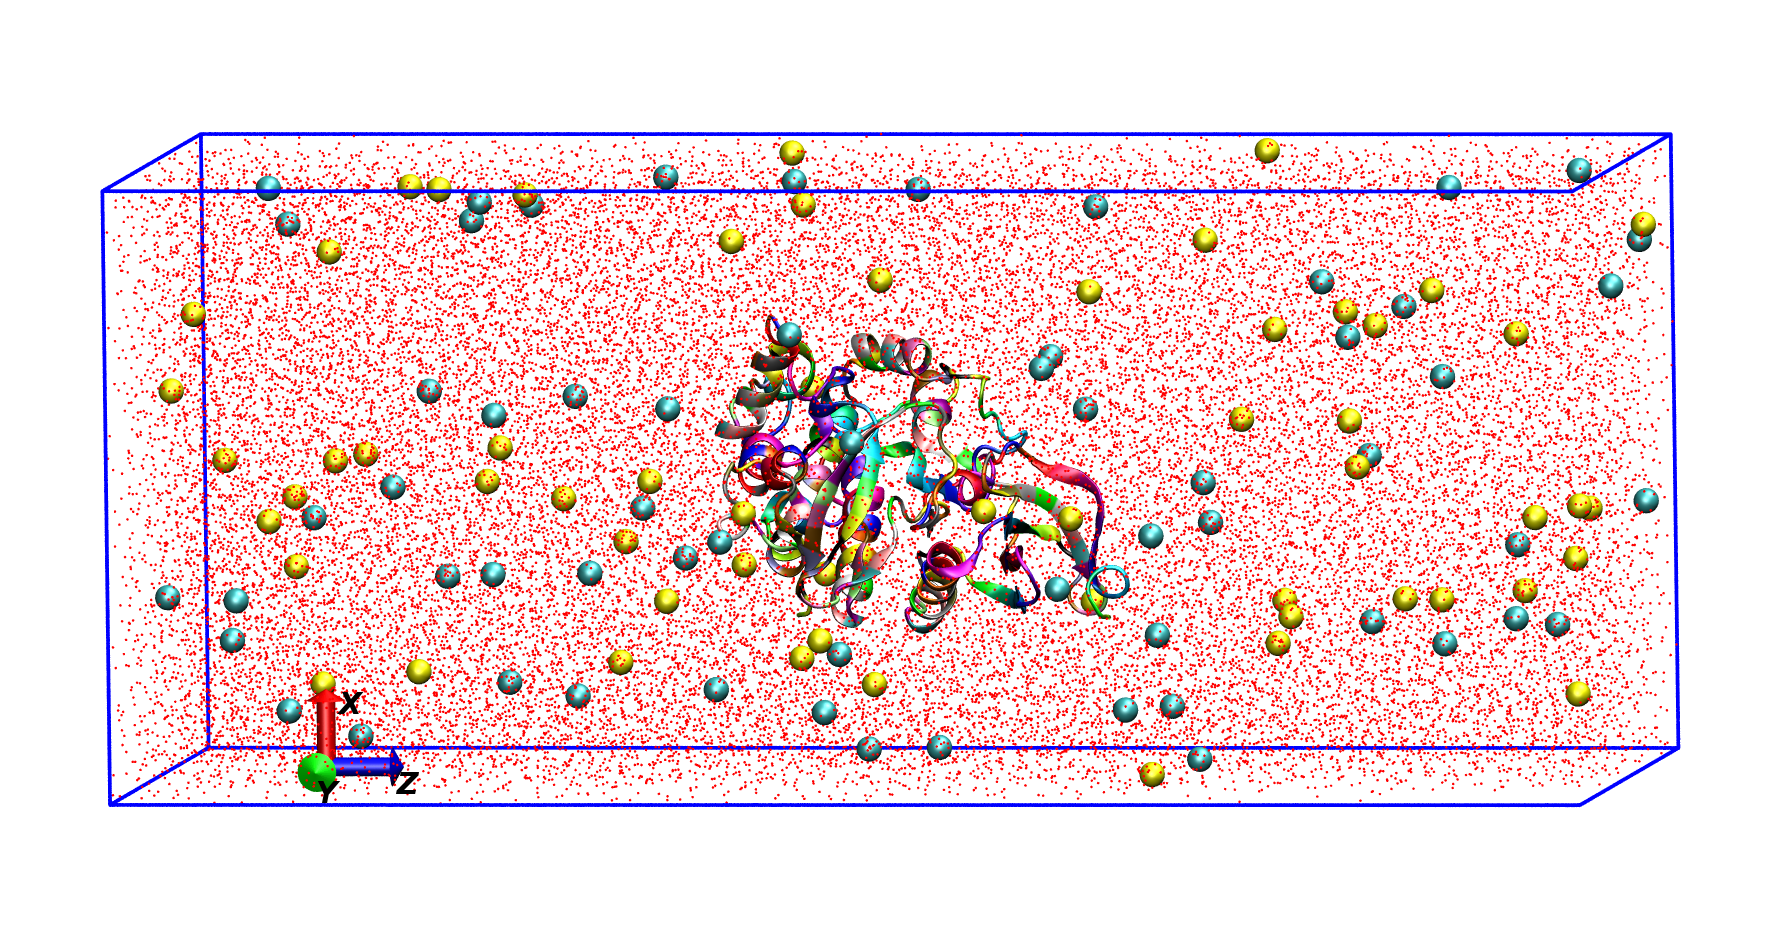
\includegraphics[width=150mm]{./rys/plot.png}
\caption{Wizualizacja symulowanego układu z białkiem, atomami tlenu od wody w kolorze czerwonym, jonami sodu w kolorze żółtym oraz jonami chloru w kolorze jasnoniebieskim.}
\end{centering}
\end{figure}

Posiadając już zrównowagowany układ można było przystąpić do właściwych symulacji rozciągania.

\section{Rozciąganie}

Rozciąganie polega na przyłożeniu wirtualnej sprężyny do środka ciężkości grupy atomów lub tak jak w tym przypadku, do pojedynczych atomów i odsuwaniu jej ze stałą szybkością. Wraz z przemieszczeniem sprężyna o zadanej stałej sprężystości $k$ powoduje powstawanie siły pomiędzy wirtualnym końcem, a danym atomem, co prowadzi do jego przemieszczenia.

Aby przystąpić do rozciągania należało zdefiniować grupy atomów, do których miała zostać przyłożona siła. Służy do tego polecenie \texttt{make\_ndx}, w którym utworzono grupy \texttt{pull} oraz \texttt{stop} z poprzednio opisanych atomów węgla alfa dwóch końcowych aminokwasów. Program \texttt{make\_ndx} posiada własną wewnętrzną składnię. Potrzebne grupy utworzono poleceniami \texttt{r 18 \& a CA} oraz \texttt{r 338 \& a CA}. Przed zapisaniem należało nadać nowo utworzonym grupom nazwy. W wyniku działania tego programu otrzymuje się plik z rozszerzeniem \texttt{.ndx}, który należy uwzględnić przy uruchamianiu \texttt{grompp} opcją \texttt{-n}.

Przy rozciąganiu najdogodniej jest stosować zespół NVE, czyli stałą liczbę cząsteczek, objętość oraz stałą energię układu. Dzięki temu mamy zagwarantowaną stałą energię układu. Wymaga to wyłączenia barostatu oraz termostatu. W tym celu potrzebna jest podwójna precyzja obliczeń. Ponadto aby zapobiec zbytniemu wzrostowi temperatury układu w wyniku obecności zewnętrznej siły, a co za tym idzie pracy, należy zastosować większe pudełko. Powyższe zmiany prowadziłyby do znacznego wydłużenia czasu obliczeń i nie zostały uwzględnione w omawianych symulacjach.

Stosując anizotropowy barostat należy uniemożliwić jego działanie w wymiarze, w którym prowadzi się rozciąganie. Bez tego pudełko ulega odbiegającym od rzeczywistości odkształceniom, mianowicie kurczy się w wymiarze, w którym badana cząsteczka ulega rozciągnięciu.

Za rozciąganie odpowiada sekcja w pliku \texttt{.mdp} zwana \textit{pull code}. Jej parametry przedstawiają się następująco:
\begin{itemize}
\item \textbf{pull} --- Odpowiada za włączenie kodu rozciągania. Opcja \texttt{constant\_force} sprawia, że rozciąganie odbywa się przy stałej sile. W tym przypadku zastosowano opcję \texttt{umbrella}, co pozwala na stosowanie stałej prędkości.
\item \textbf{pull\_geometry} --- \texttt{distance} powoduje rozciąganie wzdłuż wektora łączącego dwie grupy. Opcja \texttt{direction} umożliwia rozciąganie wzdłuż zdefiniowanego wektora. Opcja ta nakłada ograniczenie powodujące, że odległości pomiędzy dwoma rozciąganymi grupami atomów nie mogą przekroczyć połowy wymiaru, w którym zachodzi rozciąganie. Aby uniknąć tego ograniczenia stosuje się opcję \texttt{direction\_periodic}.
\item \textbf{pull\_dim} --- Określa które z wymiarów wektora siły mają być zapisywane. W tym przypadku jest to wartość siły dla osi Z układu współrzędnych.
\item \textbf{pull\_group} --- Zawiera nazwy grup atomów z pliku \texttt{ndx}, które mają zostać poddane rozciąganiu. \texttt{pull\_group0} zawiera definicję grupy odniesienia. W przypadku braku tej definicji za punkt odniesienia bierze się początek układu współrzędnych.
\item \textbf{pull\_vec} --- Definiuje wektor, wzdłuż którego białko ulega rozciąganiu odpowiednio dla każdej z grup poza grupą zerową.
\item \textbf{pull\_rate} --- Określa dla każdej z grup prędkość rozciągania. Podawana jest w pm/ns.
\item \textbf{pull\_k} --- Określa stałą siłową dla każdej z grup w kJ mol$^{-1}$ nm$^{-2}$. W opisywanych symulacjach wynosi 500 kJ mol$^{-1}$ nm$^{-2}$.
\end{itemize}

Symulacje rozciągania dla wszystkich prędkości prowadzone były na 16 rdzeniach, a każda z trajektorii była zapisywana w oddzielnym folderze. Podczas symulacji aktywny był barostat oraz termostat uprzednio używany podczas równowagowania. Rozciąganie odbywało się wzdłuż N-końca oraz C-końca białka. Jako wynik oprócz standardowych plików otrzymano pliki z wartościami siły, \texttt{pullf.xvg}.

\begin{center}
\begin{table}[h]
\centering
  \begin{tabular}{| c | l | l |}
  \hline
  Prędkość [nm/ns] & Czas symulacji [ns] & Czas obliczeń\\
  \hline
  50 & 0.2 & 1h15:55 \\
  10 & 1 & 4h48:31 \\
  5 & 2 & 11h57:22 \\
  2 & 5 & 21h50:17 \\
  0.8 & 10 & 2d7h56:25 \\
  0.4 & 20 & 3d15h07:03\\
  \hline
  \end{tabular}
  \caption{Czasy symulacji dla różnych prędkości rozciągania.}
\end{table}
\end{center}

\begin{lstlisting}[label={kod:polecenia}, caption={Polecenia Gromacsa używane  podczas symulacji podane w kolejności wykonywania}]
pdb2gmx -f hadded.pdb -o tki.gro -ignh -his
editconf -f tki.gro -o box.gro -box 8.8 7.8 7.6 -c
genbox -cp box.gro -cs spc216.gro -o water.gro -p topol.top 

grompp -f em -o ions -p topol -c water
genion -s ions -o ions.gro -p topol.top -nn 29 -np 27
grompp -f em -o em -c ions.gro -p topol
mdrun -v -deffnm em

grompp -f npt_res -o npt_res -c em.gro -p topol
mpirun -np 16 -hostfile ./hosts mdrun_mpi -v -deffnm npt_res
grompp -f npt -o npt -c npt_res.gro -p topol -e npt_res.edr -t npt_res.trr
mpirun -np 16 -hostfile ./hosts mdrun_mpi -v -deffnm npt

#### obrot czasteczki tak, by konce znalazly sie na osi Z
python rot.py
editconf -f npt_rot.gro -o npt_rot.gro -rotate 0 65.662 0
python rot.py
editconf -f npt_rot.gro -o npt_rot.gro -rotate -62.469 0 0
vmd npt_rot.gro
editconf -f npt_rot.gro -o npt_rot.gro -rotate 90 0 0
trjconv -f npt_rot.gro -o npt_large_box.gro -s npt

#### usuniecie z topol.top linii dot. wody i jonow
editconf -f npt_large_box.gro -o npt_large_box.gro -box 7.8 8.4 18.6 -c
genbox -cp npt_large_box.gro -cs spc216.gro -o npt_large_water.gro -p topol.top 
grompp -f em -o npt_large_ions -p topol -c npt_large_water
genion -s npt_large_ions -o npt_large_ions.gro -p topol.top -neutral -c 0.086

grompp -f npt_large_res -o npt_large_res -c npt_large_ions.gro -p topol
mpirun -np 16 -hostfile ./hosts mdrun_mpi -v -deffnm npt_large_res
grompp -f npt_large -o npt_large -c npt_large_res.gro -p topol -e npt_large_res.edr -t npt_large_res.trr
mpirun -np 16 -hostfile ./hosts mdrun_mpi -v -deffnm npt_large

make_ndx -f npt_large -o pull.ndx

cd p50
grompp -f pull.mdp -o pull.tpr -p ../topol.top -c ../npt_large.gro -t ../npt_large -e ../npt_large -n ../pull.ndx -maxwarn
mpirun -np 16  -machinefile ../hosts mdrun_mpi -v -s pull -dlb yes
\end{lstlisting}

\chapter{Analiza wyników}

Posiadając już dane na temat zależności siły w czasie dla różnych prędkości rozciągania można było przystąpić do analizy wyników.

\section{Znajdowanie siły rozplatania}

Pierwszym etapem był wybór z zestawu danych maksymalnej siły rozplatania. Metoda najprostsza, czyli branie jako siły rozplatania maksymalnej siły z surowych wykresów siły od rozciągnięcia ma te zalety, że jest proste i najmniej czasochłonne, niestety wynik ten byłby zakłamany w wyniku drgań termicznych, które powodują powstawanie znacznych szumów na wykresie siły od rozciągnięcia. W celu eliminacji tego niepożądanego zjawiska zastosowano wygładzanie.

Aby uzyskać wygładzone krzywe napisano skrypt w języku Python (smooth.py) w wersji 2.6.5 na systemie Ubuntu 10.04 w wersji serwerowej. Skrypt ten odpowiedzialny był za wygładzanie wykresów metodą średniej kroczącej Gaussa z zadaną szerokością ramki. Jego główną część stanowi algorytm opisany na stronie \cite{gauss}. 

Zasada jego działania polega na pobraniu liczby punktów odpowiadających szerokości ramki wokół danego punktu na wykresie niewygładzonym, a następnie wyliczeniu średniej ważonej, gdzie wagi odpowiadają rozkładowi Gaussa dla liczby punktów odpowiadających szerokości ramki.

Szerokość ramki użyta w publikacji \cite{1tki} wynosiła 0.16 nm i została użyta również w tym przypadku. Przy wygładzaniu należało uwzględnić fakt, że używana stała szerokość w nm odpowiadała różnej liczbie punktów na wykresie. Znając szybkość rozciągania oraz krok zapisu danych obliczenie liczby potrzebnych punktów stało się trywialne.

\begin{center}
\begin{figure}[h]
\begin{centering}
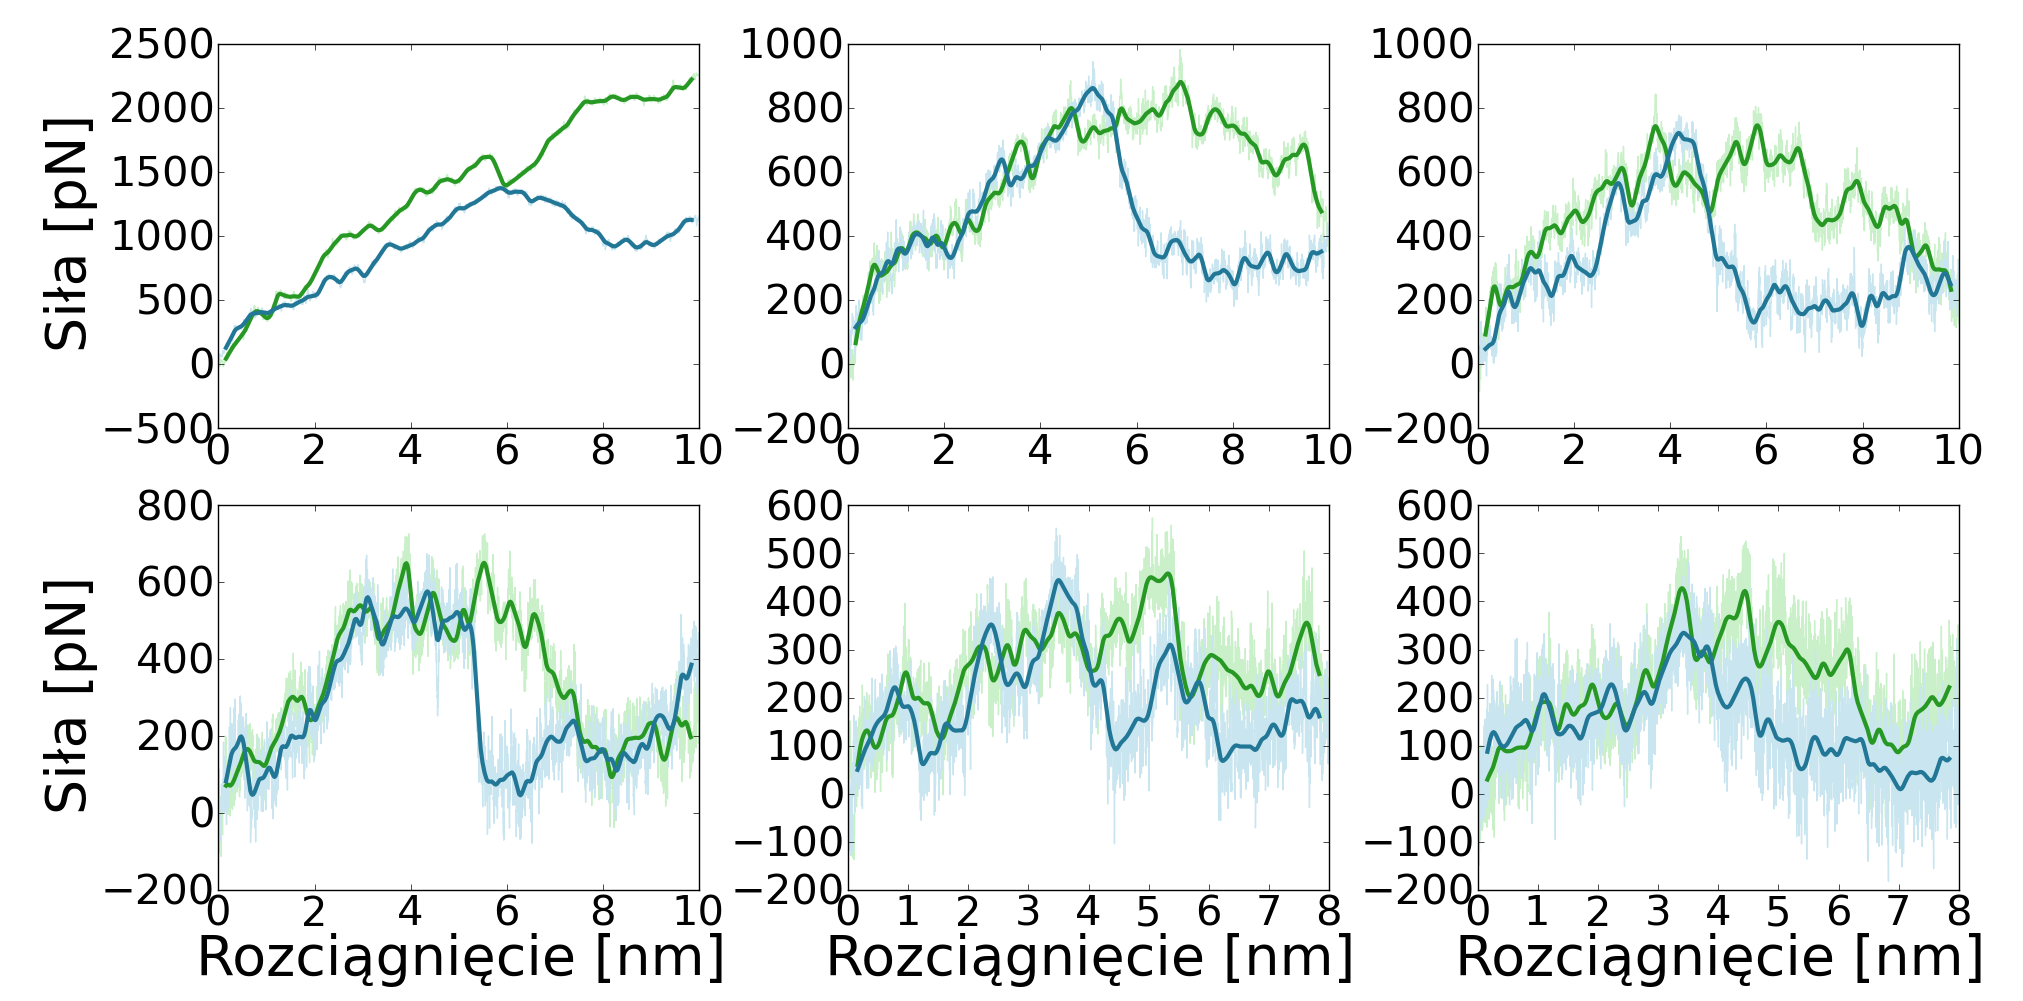
\includegraphics[width=150mm]{./rys/smooth.png}
\caption{Wygładzone krzywe zależności siły od rozciągnięcia dla 6 prędkości rozciągania dla końców białka.}
\end{centering}
\end{figure}

\end{center}

Posiadając już wygładzone wykresy siły od rozciągnięcia jako siły rozplatania bierze się maksymalne siły na wygładzonym wykresie siły od rozciągnięcia. Dla porównania z wynikami literaturowymi odczytano siły rozplatania z wykresu w publikacji \cite{1tki}.

\begin{center}
\begin{table}[h]
\centering
  \begin{tabular}{| r | c | c | c | c |}
  \hline
      & \multicolumn{4}{|c|}{Maksymalna siła [pN]} \\
\cline{2-5}
	Prędkość & \multicolumn{2}{|c|}{Z symulacji} & \multicolumn{2}{|c|}{Z publikacji} \\
\cline{2-5}
[nm/ns] &  N-koniec  & C-koniec &  N-koniec  & C-koniec \\
  \hline
  50 & 1372 & 1618  & 1323 & 1376\\
  10 & 815 & 822 & 796 & 710 \\
  5 &  720 & 745 & 645 & 526 \\
  2 & 576 & 650 &  366 & 559\\
  0.8 & 443 & 459 &  495 & 667\\
  0.4 & 334 & 429 & 452 & 538\\
  \hline
  \end{tabular}
  \caption{Maksymalne siły rozplatania dla różnych prędkości rozciągania dla symulacji oraz z danych literaturowych.}
\end{table}
\end{center}

\section{Dopasowanie krzywej teoretycznej do wyników}

\subsection{Mechanizm postępowania}

Korzystając z modelu teoretycznego Hummera--Szabo omówionego we wstępie na podstawie publikacji \cite{Hummer_Szabo_2003} oraz metodologii prezentowanej w publikacji \cite{szul} napisano skrypt w środowisku programistycznym Python, który miał za zadanie poprzez optymalizację parametrów kinetycznych znaleźć jak najlepsze dopasowanie krzywej teoretycznej dla otrzymanych wyników.

Do obliczenia teoretycznej zależności średniej siły rozplatania od prędkości rozciągania służy wzór \ref{eq:wyn} przedstawiony we wprowadzeniu.

Do optymalizacji parametrów $\mathbf{p}=\left\lbrace k_0, x_b, \kappa_m\right\rbrace$ służy funkcja najmniejszych kwadratów $S(\mathbf{p})$:

\[
S(\mathbf{p})=\sum_{i=1}^n r_i^2 
\]
\[
r_i=F_{s, i} - \overline{F}(v_i, \mathbf{p})
\]

Gdzie $F_{s,i}$ oznacza $i$-tą siłę rozplatana wziętą z symulacji dla prędkości $v_i$, a $\overline{F}(v_i, \mathbf{p})$ oznacza teoretyczną wartość siły obliczoną dla $i$-tej prędkości i parametrów $\mathbf{p}$.

Mając tak zdefiniowaną funkcję najmniejszych kwadratów minimalizuje się ją wewnętrzną funkcją \texttt{fmin()} pakietu SciPy \cite{Scipy} języka Python ze względu na parametry $\mathbf{p}$. Jest to optymalizacja metodą Simplex. Wbudowana w Pythona metoda najmniejszych kwadratów jest szybciej zbieżna niż optymalizacja metodą Simplex, jednak przy znacznej różnicy parametrów początkowych od optymalnych parametrów powoduje powstawanie błędów. Kod minimalizowanej funkcji błędu przedstawiony jest w \ref{kod:err} .
%\linespread{1}
\begin{lstlisting}[label={kod:err}, caption={Minimalizowana funkcja błędu.}]
def err(p_l):
	out=0
	fs=F(p_l,V)
	out=((fs - f)**2).sum()
	return out
p1=fmin(err, p, xtol=1e-5, maxiter=1000000, maxfun=1000000)
\end{lstlisting}

Funkcja ta pobiera parametry do optymalizacji jako lokalne \texttt{p\_l}. Na ich podstawie oraz na podstawie prędkości \texttt{V} liczona jest teoretyczna wartość siły \texttt{fs}. Suma kwadratów różnic siły teoretycznej \texttt{fs} oraz globalnej wartości siły \texttt{f} obliczana jest w linii nr 4. Do uzyskania wartości teoretycznych użyta jest funkcja \texttt{F()}, która zdefiniowana jest następująco:

\begin{lstlisting}[label={kod:F}, caption={Znajdowanie wartości funkcji teoretycznej dla zadanych parametrów i prędkości.}]

s = lambda t, vel_l, p_l: exp(-p_l[0] * exp(-0.5*ks*p_l[1]**2)/(vel_l*ks*p_l[1]*(p_l[2]/(p_l[2]+ks))**(1.5))*(exp(ks*vel_l*p_l[1]*t - (0.5*(ks*vel_l*t)**2)/(ks+p_l[2]))-1))

def F(p_l, x_l):
	k0_l, xb_l, km_l = p_l[0], p_l[1], p_l[2]
	D_l=k0_l * sqrt(2*pi) / (km_l**(1.5)*xb_l*exp(-0.5*km_l*xb_l**2))
	b=D_l*(km_l+ks)
	out=[]
	for i in range(len(x_l)):
		vel_l = x_l [i]
		a=(xb_l*D_l*(km_l+ks)**2/(ks*vel_l)+1)
		tau=(lambertW(-exp(-a))+a)/b
		out.append(-ks*300*kb*(xb_l-vel_l*quad(s,0,tau, args=(vel_l, p_l), epsabs=1e-16)[0]))
	return array(out)
\end{lstlisting}

Wartości $\overline{F}(v_i, \mathbf{p})$ stanowiące wynik równania \ref{eq:wyn} obliczane są w linii nr 13. Równania tego nie da się rozwiązać analitycznie, przez co występująca w nim całka oznaczona liczona jest numerycznie. Całka ta liczona jest dla funkcji \texttt{s} zdefiniowanej w linii nr 1, która stanowi równocześnie bezpośrednie odzwierciedlenie funkcji \ref{eq:s_t} z wprowadzenia. Granice całkowania zdefiniowane są od \texttt{0} do \texttt{tau}, które znajdywane jest na podstawie równania \ref{eq:rozw_szczeg}. Równanie to nie może być rozwiązane analitycznie, ponieważ otrzymujemy równanie typu:

\begin{equation}
a=b\tau + e^{-b\tau}
\label{eq:omega}
\end{equation} 

Gdzie \texttt{a} i \texttt{b} zdefiniowane są w kodzie. Do rozwiązania tego równania użyta została funkcja $\Omega$ Lamberta, która zdefiniowana jest jako funkcja odwrotna do $W e^W$ \cite{lambert}. Rozwiązanie równania 5.1 znalezione zostało przy pomocy programu Wolfram Alpha\cite{wolfram} i przedstawione zostało w linii nr 12 kodu. Wartości funkcji Lamberta liczone są według procedury \texttt{lambertw()}, która została zaimportowana z pakietu SciPy w wersji 0.8\cite{Scipy}.

\subsection{Analiza metody dopasowania}

Mając maksymalne siły rozplatania z symulacji oraz dysponując danymi rozplatania w tych samych warunkach tej samej cząsteczki z publikacji \cite{1tki} oraz danymi eksperymentalnymi AFM z publikacji \cite{mechanoenz}, gdzie znaleziona średnia siła rozplatania dla 1TKI wyniosła około 50 pN dla prędkości 1 $\mu$m/s można przystąpić do analizy wyników. Odbywa się ona poprzez dopasowanie parametrów  $k_0$, $x_b$ i $\kappa_m$ do danych z symulacji oraz obliczenie na podstawie tych parametrów siły rozplatania dla prędkości 1 $\mu$m/s.

Zgodnie z teorią mikroskopową przedstawioną w publikacji \cite{Hummer_Szabo_2003} krzywa teoretyczna osiąga wartości ujemne poniżej prędkości równych iloczynowi $k_0$ i $x_b$, wobec czego jeśli $k_0 x_b > 1 \mu\text{m/s}$ odzyskanie siły rozplatania jest niemożliwe.

\begin{center}
\begin{figure}[h]
\begin{centering}
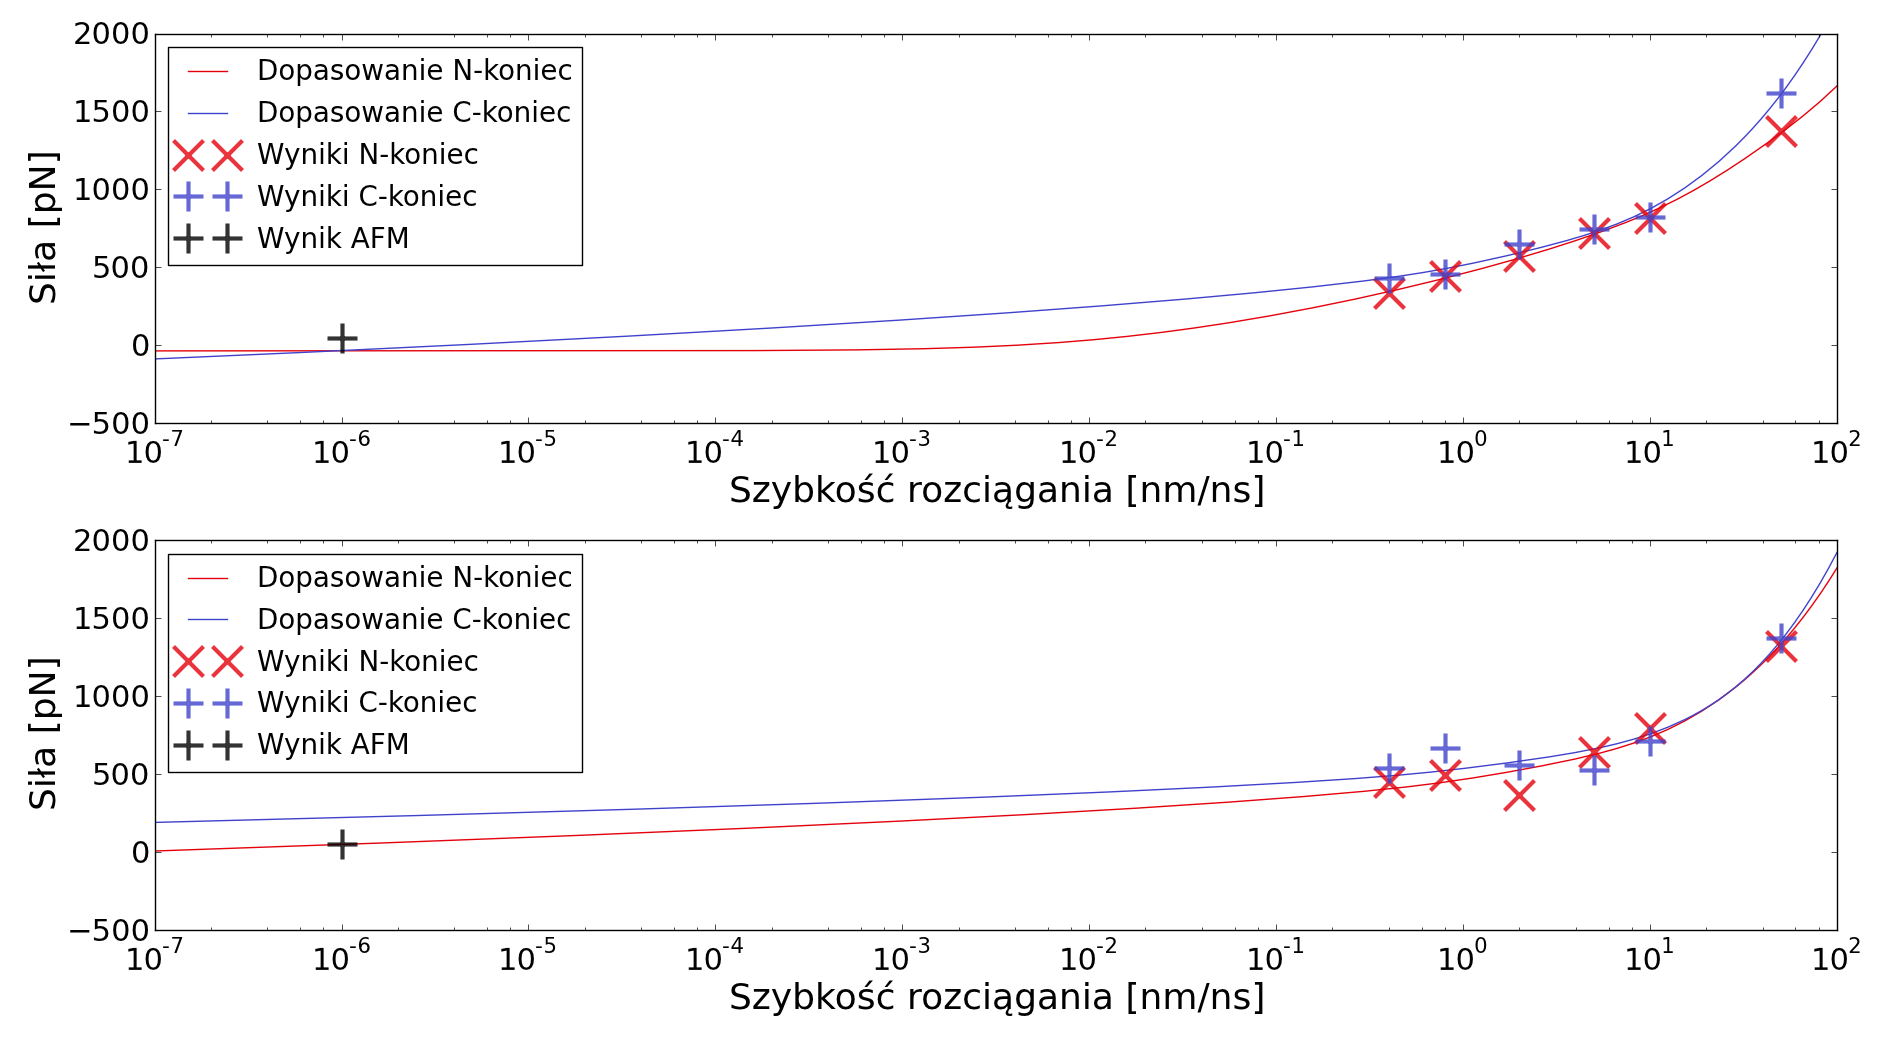
\includegraphics[width=150mm]{./rys/dop.png}
\caption{Wykresy siły rozplatania w zależności od szybkości rozciągania dla danych z symulacji (górny panel) oraz dla danych literaturowych (dolny panel) wraz z dopasowanymi krzywymi teoretycznymi.}
\end{centering}
\end{figure}
\end{center}

\begin{center}
\begin{table}[h]
\centering
  \begin{tabular}{ l l l l l}
  \hline
Koniec & $k_0$ [s$^{-1}$] & $x_b$ [nm] & $k_bT\kappa_m$ [N/m] & $x_b k_0$ [m/s] \\
  \hline
Symulacje \\
N & 7.944\e{7} & 0.04287& 38.36 & 3.41\e{-3} \\
C & 2.787\e{3} & 0.1960 & 3.669 & 4.56\e{-7} \\
\hline
Praca \cite{1tki}\\
N & 3.970\e{-1}& 0.347 & 1.804 & 1.38\e{-10} \\
C & 1.219\e{-26} & 1.101 & 0.5820 & 1.34\e{-35}\\
\hline
  \hline
  \end{tabular}
  \label{tab1}
  \caption{Parametry kinetyczne $k_0$, $x_b$ i $\kappa_m$ dla N i C-końca 1TKI z symulacji i z publikacji \cite{1tki}}
\end{table}
\end{center}

Z tabeli 5.2 wynika, że jedynie w przypadku parametrów odzyskanych z symulacji rozciągania dla N-końca dla publikacji \cite{1tki} sensowna jest próba odzyskania siły rozplatania dla prędkości 1$\mu$m/s. Dla tych parametrów wynosi ona 48.9 pN, co jest dość dobrym przybliżeniem wobec 50 pN eksperymentalnych. 

Zbadano również zależność uzyskiwanych parametrów kinetycznych od wyboru punktu startowego. Analizę tę wykonano dla danych pochodzących z symulacji dla C-końca.

\begin{center}
\begin{table}[h!]
\centering
  \begin{tabular}{ | l l l l l l l l l |}
  \hline
Parametr & & & & & & & & \\
\hline
$k_0$ 1.6$\times$ [s$^{-1}$] & 10$^{-17}$ \cellcolor{red}&10$^{-16}$ \cellcolor{green}& 10$^{-12}$ \cellcolor{green}& 10$^{-2}$ \cellcolor{green}& 10$^{2}$ \cellcolor{green}& 10$^{8}$ \cellcolor{green}& 10$^{10}$ \cellcolor{red} & 10$^{12}$ \cellcolor{red}\\
$x_b$ \e{-10}[m] & 0.5 \cellcolor{red}& 1 \cellcolor{green}& 2 \cellcolor{green}& 4 \cellcolor{green}& 6 \cellcolor{green}& 8 \cellcolor{green}& 10 \cellcolor{green}& 20 \cellcolor{red}\\
$\kappa_m$ \e{20} & 0.5\cellcolor{red} & 1\cellcolor{red} & 2 \cellcolor{green}& 3 \cellcolor{green}& 4 \cellcolor{green}& 4\e{22} \cellcolor{green}& 4\e{23}\cellcolor{red} & 4\e{24}\cellcolor{red}\\
\hline
  \end{tabular}
  \label{tab1}
  \caption{Startowe parametry kinetyczne $k_0$, $x_b$ i $\kappa_m$ dla N-końca. Na czerwono zaznaczono te parametry, które generowały błąd.}
\end{table}
\end{center}

W tabeli 5.3 umieszczono przykładowe parametry startowe. Na czerwono zaznaczono te, dla których optymalizacja nie powiodła się. Parametry startowe zaznaczone na zielono doprowadziły w wyniku optymalizacji do tych samych wartości, co przedstawione w tabeli 5.2. 

Do dopasowania brane były wyniki pojedynczych symulacji, co przy dopasowaniu do wykresu \textbf{średnich} sił zerwania mogło prowadzić do dużych błędów w otrzymanych parametrach kinetycznych. Aby sprawdzić wpływ błędów wyników symulacji zbadano wpływ $\pm$10\% wartości siły rozplatania dla najwyższej i najwolniejszej szybkości rozplatania dla danych z symulacji dla C-końca na wartości odzyskanych parametrów kinetycznych.

\begin{center}
\begin{table}[h!]
\centering
  \begin{tabular}{ l l l l l l}
  \hline
 & $k_0$ [s$^{-1}$] & $x_b$ [nm] & $k_bT\kappa_m$ [N/m] & $x_b k_0$ [m/s] & $\sum r^2 $\\
  \hline
Symulacja & 2.787\e{3} & 0.1960 & 3.669 & 4.56\e{-7} & 7.604\e{-21} \\
 $v=$50 m/s\\
 +10\% & 1.700\e{-5} & 0.4914 & 1.224 & 8.35\e{-15} & 1.165\e{-20}\\
 --10\% & 3.500\e{4} & 0.1499 & 5.492 & 5.25\e{-6} & 5.863\e{-21} \\
 \hline
 $v=$0.4 m/s\\
+10\% & 2.152 & 0.2929 & 2.340 & 6.30\e{-10} & 8.00\e{-21}\\
--10\% & 8.289\e{4} & 0.1503 & 4.987 & 1.25\e{-5} & 8.91\e{-21}\\
\hline
 \hline
  \end{tabular}
  \label{tab1}
  \caption{Zmiany wyznaczonych parametrów kinetycznych w zależności od zmiany wartości maksymalnych sił rozplatania.}
\end{table}
\end{center}

Z tabeli 5.4 wynika, że zmiana wyników o 10\% prowadzi do zmiany $k_0$ o kilka rzędów wielkości.

Sprawdzono również tę metodę dla wyników symulacji rozciągania innego białka, modułu tytyny I91\cite{Tit_I91}, 1TIT w bazie PDB. Wyniki te były wzięte z pracy \cite{szul}, gdzie parametry kinetyczne były wybierane nie na drodze numerycznej optymalizacji, ale za pomocą analizy dopasowania różnych zestawów parametrów. W przypadku tego białka dysponowano również zestawem parametrów kinetycznych $k_0$ i $x_b$ z eksperymentów AFM z pracy\cite{carr}, przy czym przy braku $\kappa_m$ uzyskane ono zostało z dopasowania do danych eksperymentalnych i z symulacji przy stałych pozostałych parametrach.

\begin{table}[H]
\centering
  \begin{tabular}{ l l l l l l}
  \hline
 & $k_0$ [s$^{-1}$] & $x_b$ [nm] & $k_bT\kappa_m$ [N/m] & $x_b k_0$ [m/s] & $\sum r^2 $\\
  \hline
Dopasowanie & 7.7\e{-1} & 0.172 & 7.52 & 1.32\e{-10} & 2.65\e{-21}\\
Praca\cite{szul} & 1.6\e{-11} & 0.385 & 2.86 & 6.16\e{-21} & 1.17\e{-20} \\
AFM\cite{carr} & 3.3\e{-4}& 0.250 & 4.54 & 8.25\e{-14} & 9.27\e{-21}\\


\hline
 \hline
  \end{tabular}
  \label{tab1}
  \caption{Dopasowanie parametrów kinetycznych do danych z pracy \cite{szul}, przedstawienie parametrów z \cite{szul} oraz parametrów kinetycznych z eksperymentu AFM \cite{carr}}
\end{table}

\begin{figure}[H]
\begin{centering}
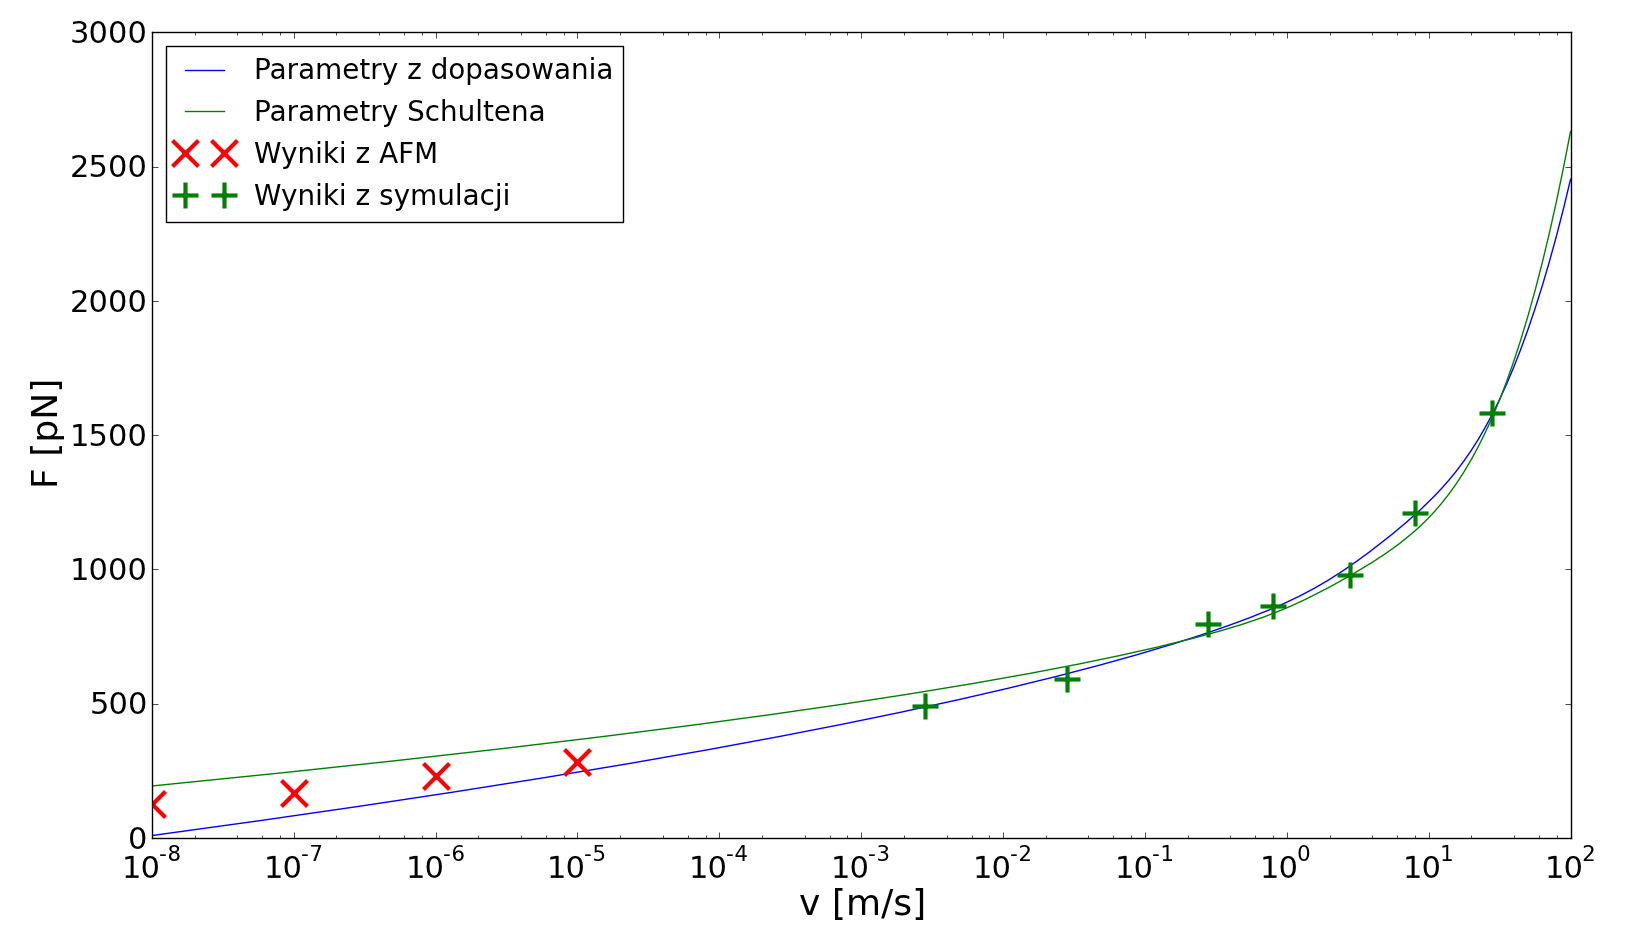
\includegraphics[width=150mm]{./rys/dop_schul.png}
\caption{Wykres krzywej teoretycznej z parametrami z pracy Schultena oraz po dopasowaniu z naniesionymi danymi z eksperymentu AFM.}
\end{centering}
\end{figure}

\begin{table}[H]
\centering
  \begin{tabular}{ l c c c c}
  & F [pN]\\
  \hline
 v [nm/ms]& AFM  & Praca\cite{szul} & Z dopasowania\\
  \hline
0.01 & 125 &  193 & 8.6 \\
0.1 & 166 &  247 & 82 \\
1 & 230 &  304 & 160\\
10 & 283 &  366 & 244\\

\hline
 \hline
  \end{tabular}
  \label{tab1}
  \caption{Przedstawienie sił rozplatania wyliczonych z dopasowania do danych z symulacji w porównaniu do rzeczywistych średnich sił rozplatania zmierzonych w eksperymencie AFM.}
\end{table}

Przy czym zmiana średniej siły zerwania dla v=2.8 m/s z 997 pN na 978 pN czyli o 1.9\% spowodowała zmianę dopasowania $k_0$ o rząd wielkości i zmianę wyznaczanej siły dla prędkości 0.01 nm/ms z 2\e{-2} pN do 8.6 pN.

\section{Analiza wydajności klastra}

Pierwszym etapem w analizie wydajności było zbadanie jakości połączenia realizowanego pomiędzy dwoma komputerami. Komunikacja pomiędzy nimi odbywała się poprzez sieć 1 Gbps, jednak komputery te zostały wyposażone w 2 karty, także teoretyczna przepustowość powinna wynosić 2 Gbps. 

Do analizy wydajności sieci służy narzędzie NetPIPE \cite{netpipe}. 

Analizę przepustowości przeprowadzono zarówno na pojedynczych kartach jak i na obu kartach działających razem.

\begin{center}
\begin{figure}[h]
\begin{centering}
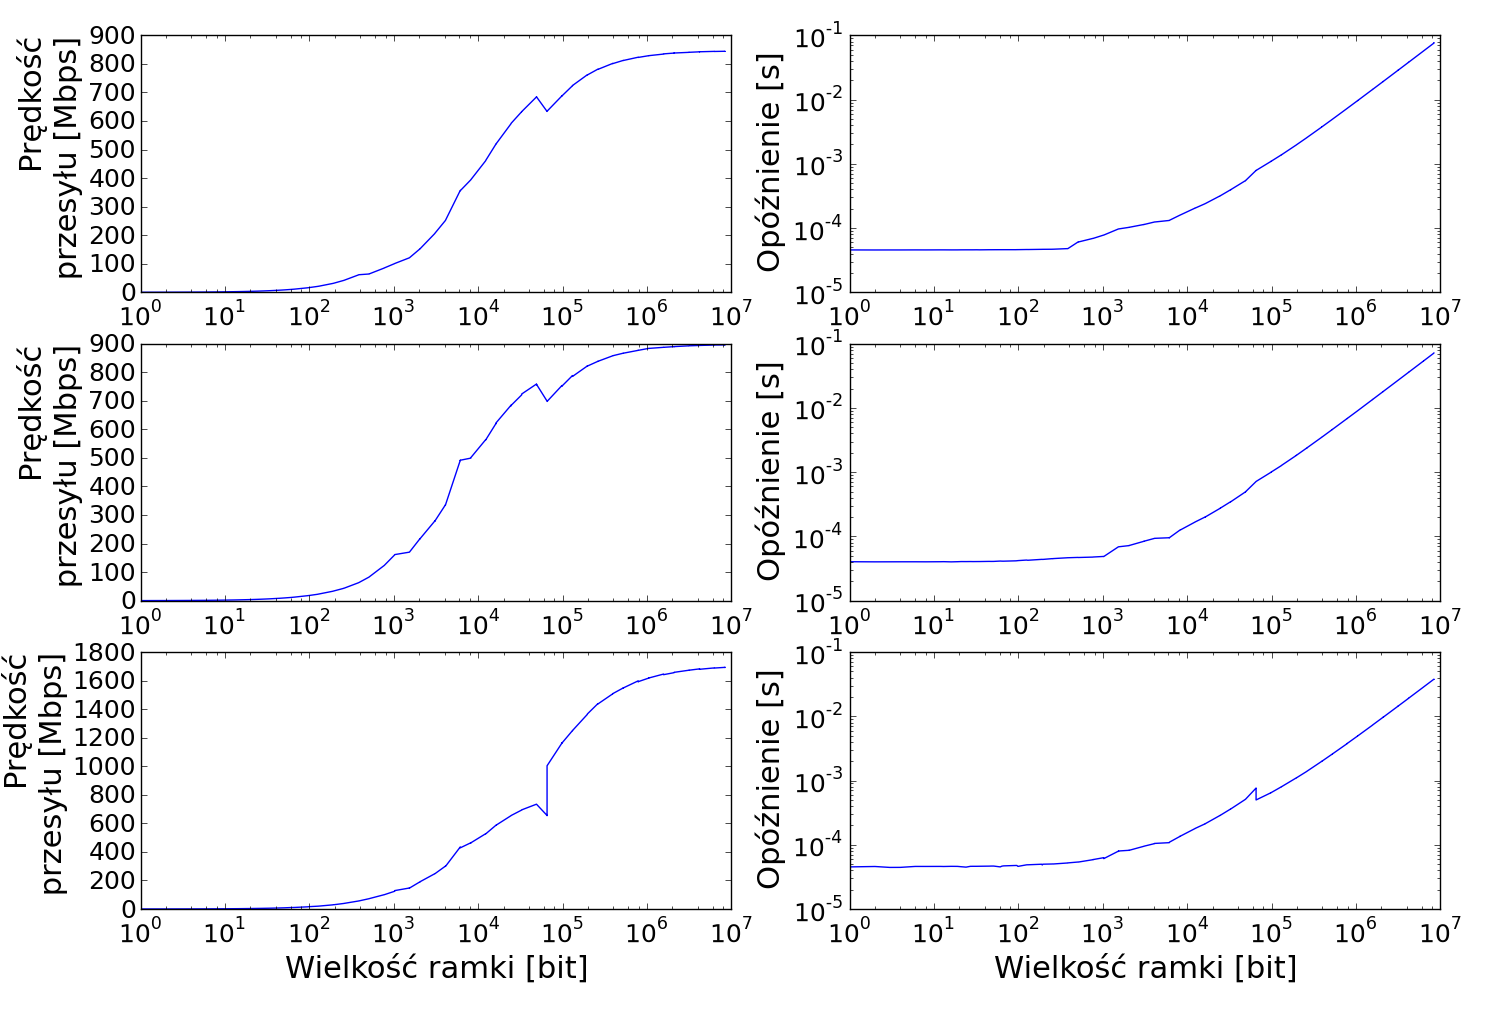
\includegraphics[width=150mm]{./rys/speed.png}
\caption{Wykresy przepustowości oraz opóźnienia dla poszczególnych kart sieciowych oraz dla kart sieciowych działających razem w zależności od wielkości przesyłanych danych.}
\end{centering}
\end{figure}
\end{center}

Na podstawie wykresów można odczytać, że przepustowość komunikacji MPI przez pierwszą jak i przez drugą kartę sieciową wynosi odpowiednio 830 Mbps oraz 890 Mbps. Po włączeniu obu kart sieciowych naraz przepustowość komunikacji rośnie do 1680 Mbps. Opóźnienia dla małych rozmiarów pakietów wynoszą odpowiednio 42 $\mu$s oraz 36 $\mu$s. Dla kart działających razem opóźnienie to wynosi około 45 $\mu$s.

Wyniki te świadczą o wydajnym połączeniu pomiędzy dwoma komputerami, jednak opóźnienia rzędu kilkudziesięciu $\mu$s nijak mają się do tych osiąganych przez sieci typu Infiniband czy też Myrinet, które są o rząd wielkości mniejsze, co pozwala na zmniejszenie opóźnień w komunikacji pomiędzy procesami i w efekcie prowadzi do lepszej skalowalności.

Analiza wydajności klastra polegała na wykonaniu tej samej powtórzonej symulacji na różnej liczby rdzeni, a następnie zbadaniu czasu potrzebnego na obliczenia w zależności od liczby wykorzystywanych rdzeni. Dobrym wyznacznikiem jest liczba ns obliczonych w określonej jednostce czasu, na przykład na dzień. W idealnym przypadku liczba ta powinna rosnąć liniowo wraz ze wzrostem liczby wykorzystywanych rdzeni. 

Do symulacji użyto tego samego układu, który był rozciągany przy prędkości 50~nm/ns. Symulację powtarzano 16 razy idąc od obliczeń na 1 rdzeniu aż do obliczeń na 16 rdzeniach prowadzonych równolegle. Obliczenia te wykonano zarówno z użyciem przydziału osobnych rdzeni na obliczenia PME jak i bez. Powyżej 8 rdzeni komunikacja między komputerami odbywała się poprzez dwie karty 1Gbps. 

Na tej podstawie sporządzono wykresy wydajności liczonych ns/dzień oraz porównano jak obliczona wydajność ma się w stosunku do teoretycznego liniowego wzrostu wydajności. 

\begin{center}
\begin{figure}[h!]
\begin{centering}
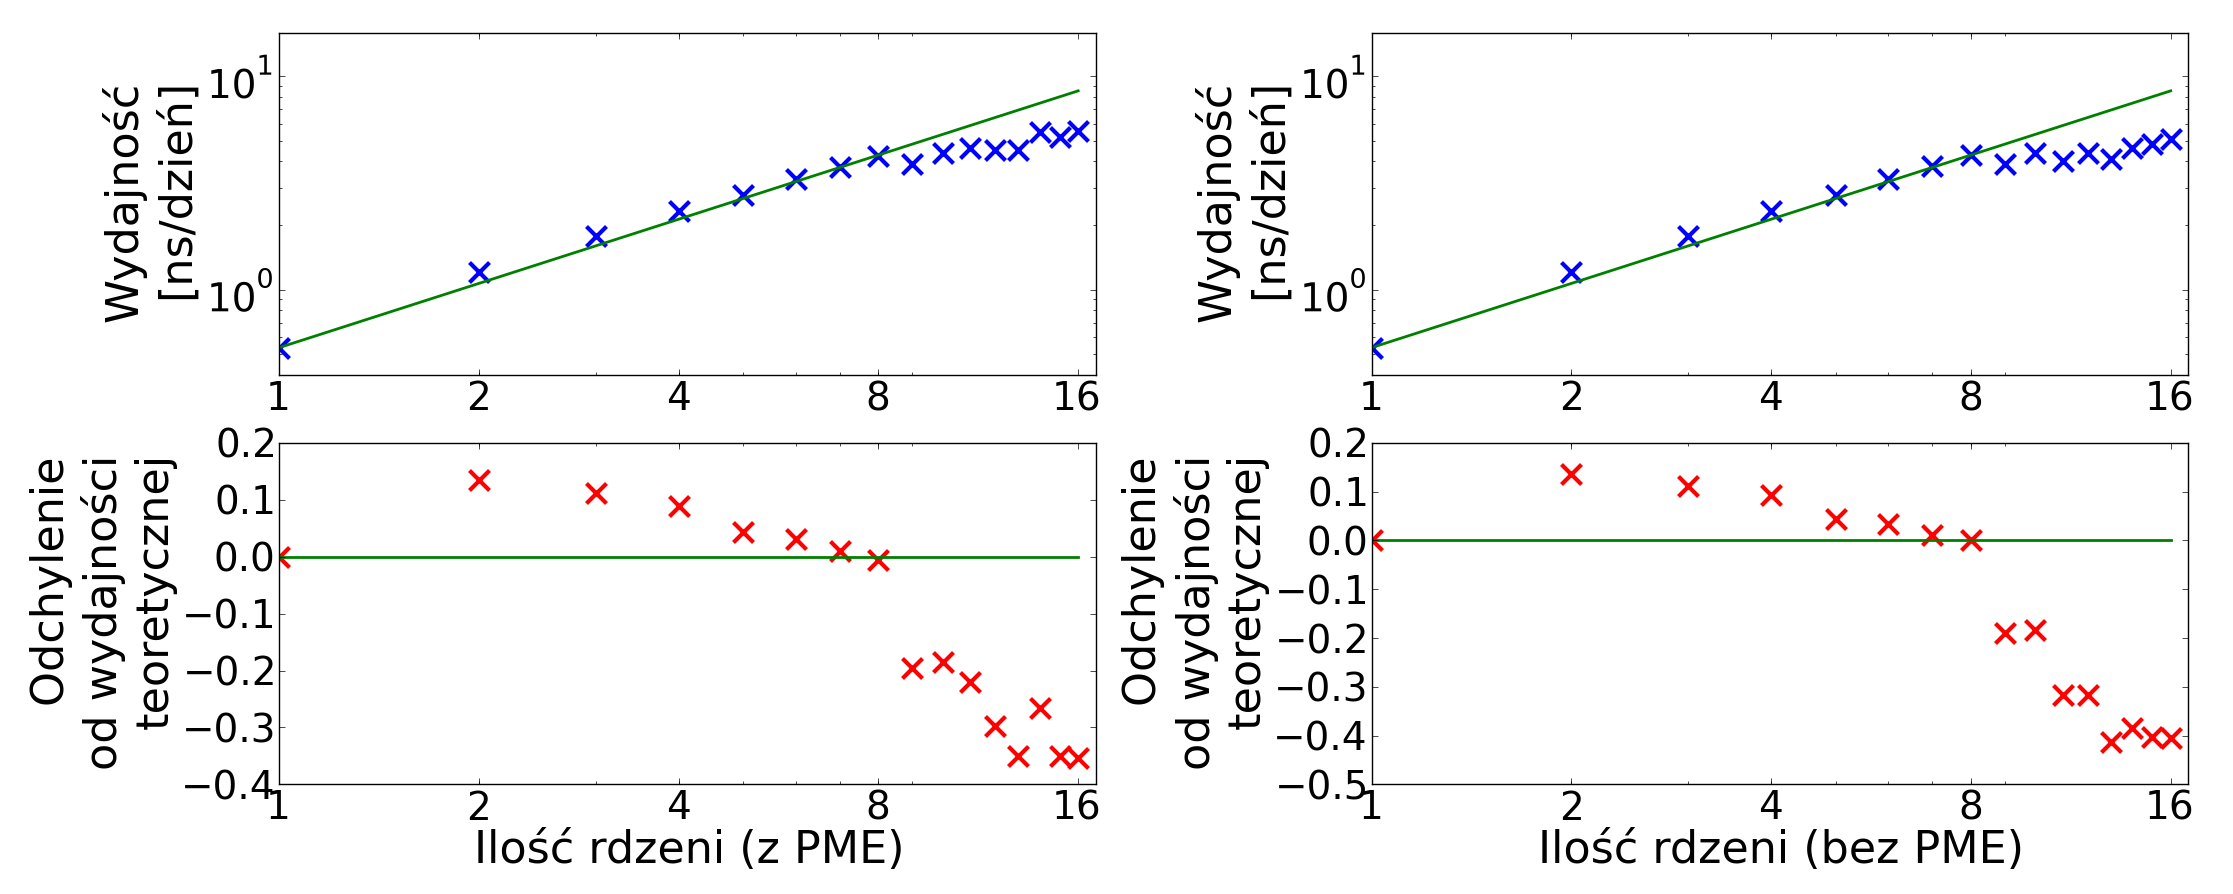
\includegraphics[width=150mm]{./rys/wyd.png}
\caption{Wykres wydajności obliczeń w zależności od liczby użytych rdzeni oraz ich odchyleń od wartości teoretycznych.}
\end{centering}
\end{figure}
\end{center}

Z powyższych wykresów można wnioskować, że skalowalność klastra zachowuje się liniowo aż do bariery 8 rdzeni. Ponadto wydajność obliczeń powyżej 1 rdzenia rośnie powyżej zależności teoretycznej, co świadczy o tym, że obliczenia tylko na jednym rdzeniu są wolniejsze. Po przekroczeniu granicy obliczeń prowadzonych na 8 rdzeniach wydajność w najgorszym przypadku jest o około 40\% mniejsza niż wynikałoby to z linowego wzrostu wydajności. Podobne wyniki dają obliczenia prowadzone przy automatycznym wyborze liczby rdzeni przeznaczonych tylko na obliczenia PME jak i obliczenia prowadzone bez przydziału osobnych rdzeni na obliczenia PME poprzez zastosowanie opcji \texttt{-nopme} w programie \texttt{mdrun}.

Wydajność obliczeń w przypadku zastosowania automatycznego przydziału rdzeni na obliczenia PME jest jednak wyraźnie większa przy wykorzystaniu 16 rdzeni niż bez tego przydziału. 

\chapter{Wnioski}

Na podstawie przeprowadzonych obliczeń można wywnioskować, że symulacje rozplatania białek o znanej strukturze mogą być pomocne przy odzyskiwaniu parametrów kinetycznych. Należy jednak zawsze pamiętać, że metoda ta może być tylko wspomaganiem eksperymentu. Ostatecznym potwierdzeniem zawsze musi być emipryczny, dający się powtórzyć wynik doświadczalny, a nie tylko teoretyczny. 

Dokładność uzyskanych parametrów kinetycznych w ogromnej mierze zależy od ilości oraz jakości uzyskanych wyników symulacji. Stosując dużą próbę statystyczną uzyskujemy lepsze wyniki. Pojedyncze wartości sił rozplatania czy też zerwania stanowią zbyt słabą przesłankę co do prawdziwości odzyskanych parametrów kinetycznych. Ponadto w celu poprawnego dopasowania ogromny wpływ ma także duża rozpiętość badanych szybkości. Im więcej, tym lepiej. Badana zależność sił rozplatania od prędkości rozciągania ma jednak charakter logarytmiczny. Pociąga to za sobą wykładniczy wzrost czasu potrzebnego do symulacji, a co za tym idzie czasu obliczeń. Z tego powodu zachodzi potrzeba zakupu coraz to wydajniejszego sprzętu. 

Pojedyncze wyniki, tak jak w tym przypadku powodują powstawanie dużego błędu z powodu małej liczebności grupy. Oznaczane parametry, jak na przykład stała rozplatania $k_{0}$ charakteryzują się dużą czułością i nawet błąd kilkudziesięciu pN w oznaczaniu siły rozplatania może oznaczać różnice wyznaczonej stałej szybkości sięgającą kilku rzędów wielkości. Nie tyle rozwiązaniem, co ograniczeniem tego problemu jest wspomniane wcześniej zwiększenie próby, co pociąga za sobą jednak zwiększenie czasu obliczeń. Za pociesznie może jednak służyć fakt, że rozrzut sił rozplatania maleje wraz ze spadkiem prędkości. Z drugiej strony jednak dokładność uzyskanych parametrów kinetycznych zależy przede wszystkim od wartości dla mniejszych prędkości.

Przy odzyskanych parametrach kinetycznych obliczone na ich podstawie siły dla eksperymentalnego zakresu prędkości znacząco odbiegają od tych wyznaczonych doświadczalnie. Wynika to z czułości algorytmu dopasowania na wyniki symulacji. Ponadto ekstrapolacja sił rozplatania dla zakresu eksperymentalnego jest bardzo czuła na zmiany parametrów kinetycznych, które dla zmiany sił rozplatania o 10\% mogą przyjmować wartości różniące się od siebie nawet o kilka rzędów wielkości. Dlatego też metoda ta wymaga dalszego doskonalenia. Przy większej liczbie wyników symulacji dla danej szybkości pomocne może być uwzględnienie odchyleń standardowych przy metodzie najmniejszych kwadratów poprzez stosowanie ważenia. Wymaga to jednak większej ilości wartości sił rozplatania dla danej szybkości.

Budowa klastra na zwykłej sieci o przepustowości 1 Gbps opartej na zwykłym switchu przy maszynach wieloprocesorowych, kiedy to na jednej maszynie może być uruchomionych aż 8 niezależnych procesów jest nieefektywna. Ze względu na niewielki wzrost wydajności przy użyciu wszystkich 16 wątków rozsądniejsze wydaje się prowadzenie obliczeń równolegle na dwóch maszynach. Wynika to z prostego faktu, że komunikacja pomiędzy procesami uruchomionymi na jednej płycie głównej jest nieporównywalnie szybsza niż pomiędzy tymi samymi procesami połączonymi przez sieć. W zastosowaniu znajdują się specjalne szybsze łącza typu Infiniband czy Myrinet, które pozwalają na uzyskanie lepszej skalowalności. 

Nie można także zapominać o wiedzy potrzebnej do prawidłowej obsługi programów do symulacji dynamiki molekularnej. W przypadku programu Gromacs opanowanie parametrów służących do kontroli symulacji zajęło około rok bazując przede wszystkim na znalezionych w internecie samouczkach oraz listach mailingowych służących do wymiany myśli pomiędzy użytkownikami. Dlatego też dobór takich opcji jak czas równowagowania, sprotonowanie, zespół, typ barostatu i termostatu ma kluczowy wpływ na wynik. Nieznajomość parametrów, a co za tym idzie nieumiejętność ich kontroli może prowadzić do sytuacji, kiedy to wynik symulacji nie ma nic wspólnego z rzeczywistością. Nawet będąc pewnym swoich umiejętności zawsze należy podchodzić do wyniku symulacji z dużą rezerwą, ponieważ jest to tylko wynik teoretyczny. 

Symulacje dynamiki molekularnej stanowią ogromną wartość jako narzędzie do badania i wizualizacji procesów odbywających się w skali pojedynczej cząsteczki. Dzięki temu mamy możliwość wglądu na zachowanie oraz rolę poszczególnych atomów w trakcie danego procesu. 
\clearpage
\addcontentsline{toc}{chapter}{Bibliografia}
\newpage
\bibliography{b}
\newpage 
\clearpage
\addcontentsline{toc}{chapter}{Dodatek A. Spis zawartości dołączonej płyty CD}
\chapter*{Dodatek A. Spis zawartości dołączonej płyty CD}

\dirtree{%
.0 Katalog główny.
.1 praca.pdf - Praca magisterska.
.1 smooth.py - Skrypt Pythona odpowiedzialny za wygładzanie.
.1 fit\_polaczone.py - Skrypt Pythona odpowiedzialny za dopasowanie modelu Hummera-Szabo do danych.
.1 README - Plik z opisem zawartości płyty.
.1 pliki\_Gromacs - Katalog z plikami potrzebnymi do przeprowadzenia symulacji.
.2 polecenia - Spis poleceń Gromacsa używanych przy symulacji.
.2 1TKI.pdb - Oryginalny plik PDB z bazy danych.
.2 hadded.pdb - Plik PDB po operacjach programem WHATIF.
.2 rot.py - Skrypt Pythona do obliczania kątów przy obracaniu białka.
.2 hosts - Plik z adresami hostów dla OpenMPI.
.2 topol.top - Plik topologii.
.2 *.mdp - Pliki z parametrami dla równowagowania.
.2 p50 - parametry i podsumowanie dla v=50 nm/ns.
.3 pull.mdp - Parametry dla rozciągania.
.3 md.log - Informacje na temat symulacji.
.2 p10 - parametry i podsumowanie dla v=10 nm/ns.
.2 p5 - parametry i podsumowanie dla v=5 nm/ns.
.2 p2 - parametry i podsumowanie dla v=2 nm/ns.
.2 p0.8 - parametry i podsumowanie dla v=0.8 nm/ns.
.2 p0.4 - parametry i podsumowanie dla v=0.4 nm/ns.
}

\newpage
\thispagestyle{empty}
\mbox{}
\newpage
\thispagestyle{empty}
\begin{singlespace}
\setlength{\parskip}{0.5cm}
\setlength{\parindent}{0pt}
\begin{flushright}
Poznań, dnia \today{}
\end{flushright}
% \vspace{0.5cm}
\begin{center} 
\LARGE{OŚWIADCZENIE}
\end{center}
\vspace{0.5cm}
Ja, niżej podpisany \textbf{Mateusz Najsztub}, student Wydziału Chemii Uniwersytetu im. Adama Mickiewicza w Poznaniu oświadczam, że przedkładaną pracę dyplomową pt.: 

%\textbf{``Rozciąganie cząsteczek wielomodułowych - symulacje i analiza danych''}
$\dots\dots\dots\dots\dots\dots\dots\dots\dots\dots\dots\dots\dots\dots\dots\dots\dots\dots\dots\dots\dots\dots\dots\dots\dots\dots\dots$

$\dots\dots\dots\dots\dots\dots\dots\dots\dots\dots\dots\dots\dots\dots\dots\dots\dots\dots\dots\dots\dots\dots\dots\dots\dots\dots\dots$

napisałem samodzielnie. Oznacza to, że przy pisaniu pracy, poza niezbędnymi konsultacjami, nie korzystałem z pomocy innych osób, a w szczególności nie zlecałem opracowania rozprawy lub jej części innym osobom, ani nie odpisywałem tej rozprawy lub jej części od innych osób. 

Oświadczam również, że egzemplarz pracy dyplomowej w formie wydruku komputerowego jest zgodny z egzemplarzem pracy dyplomowej w formie elektronicznej.

Jednocześnie przyjmuję do wiadomości, że gdyby powyższe oświadczenie okazało się nieprawdziwe, decyzja o wydaniu dyplomu zostanie cofnięta.
\vspace{0.5cm}
\begin{center}
\begin{tabular}{p{10 cm} p{10cm}}
Prof. dr hab. Andrzej Molski & $\dots\dots\dots\dots\dots\dots\dots\dots\dots$\\
/nazwisko kierownika pracy magisterskiej/ & /podpis studenta/\\
& \\
& \\
$\dots\dots\dots\dots\dots\dots\dots\dots\dots\dots$ & 87102302630\\
/podpis kierownika pracy magisterskiej/ & /PESEL studenta/
\end{tabular}

%\setlength{\parskip}{1cm}
%\vspace{2cm}

\end{center}
\end{singlespace}


\end{document}
